%! Author = danjane
%! Date = 17.09.22

\documentclass[10pt]{article}

\usepackage{amsmath, amsfonts}
\usepackage{cmbright}

\usepackage{tcolorbox}
\usepackage{adjustbox}
\usepackage{pdflscape}
\usepackage{graphicx}
\usepackage{hyperref}

\usepackage{tikz}
\usetikzlibrary{positioning}
\tikzset{
  desk/.style={
    shape=rectangle,
    draw,
    font=\footnotesize,
    minimum width=2cm,
    minimum height=1cm,
  },
  block/.style={
  draw, rectangle, minimum height=1cm
  }
}

\usepackage{listings}
\lstset{
    language=Python,
%    basicstyle=\scriptsize,
    numbers=left,
}

\begin{document}

\begin{titlepage}
\large

\centering

{\Huge TAT: teacher assisting tools}

\vspace{5mm}

{\Large An application to manage teacher-student interactions}

\vfill
{\Large James Daniel Trevarton Jane}

\vspace{5mm}

August 2023

\vfill
supervised by

Dr.~Pierre-Alain Cherix
\vfill


\url{https://github.com/danjane/GymInf}


\makebox[\textwidth][c]{
\includegraphics[width=1.4\textwidth]{GymInfBanner.png}}

\end{titlepage}

\tableofcontents

\section*{Acknowledgements}

A big thank you to Pierre-Alain Cherix for his suggestions and advice. His years of experience with computers, teaching and teachers led to a very different, and much better, project than I had first envisaged.

Thanks to Chris Lawrence for discussions about test-driven development, Pat Jane for hilarious stories of systems design disasters, and Ruskin Constant for the basics of UX. I also thank my family: Sarah for her support, and Gabriel and Julia for destruction testing the GUI (and everything else in the house). 

\newpage
\section{Introduction}

From the classic teaching literature, Bucheton and Soulé have described the act of teaching as a multi-agenda game of postures requiring good preparation and excellent micro-decisions \cite{BS09}. In their model, they identify the crucial roles of the teacher in controlling the cadence, the atmosphere, the scaffolding and the relationships during the class, and how each supports the learning objective. Many of the teacher's most time-consuming tasks do not take place in the classroom: good preparation and strong follow-ups (auto-reflection, marking, parent-teacher interactions) work to support and complement the overall success of the student learning process.

For example, scanning the offers of teaching posts we see that teacher responsibilities include the ability to
\begin{itemize}
\item plan and implement effective classroom management practices,
\item design and implement effective strategies to develop independent learners,
\item engage students in active, hands-on, creative problem-based learning,
\item build students’ ability to work collaboratively with others,
\item maintain a safe, orderly environment conducive to learning,
\item adapt instruction/support to students’ differences in development, learning styles, strengths and needs, and
\item write student reports to guide changes in instruction and practice, and to improve student learning.
\end{itemize}

As A. Sweigart points out in his 2015 book "Automate the boring stuff" many of the teaching tasks listed above are ripe for automation \cite{Swei15}. I would also accept that some of these tasks should \textbf{not} be automated (even if they can be). As John Hattie explains in \emph{Visible Learning} \cite{Hat12}, \emph{``Expert teachers monitor learning and provide feedback.''} In my opinion writing student reports are a perfect example of a necessary evil: although time consuming (and potentially stressful) for the teacher, writing a student report forces the teacher to reflect on the progress of the student and at the same time manage the expectations of all partners - student, teacher, management and parent.

So which tasks should be automated? Why? And for whom? When I first started teaching, my natural character led to two bad teaching practices: I found it difficult to engage with the quieter, more reserved students; and I was so busy answering student questions that I left little time for taking notes. I felt my teaching (and so hopefully also my students' learning experience) would benefit from a tool which tracked my interactions in class in an attempt to shift the focus away from the "louder" students. 
\begin{center} 
\emph{``The best climate for learning is one in which there is trust. Students often don’t like to make mistakes because they fear a negative response from peers. Expert teachers create classrooms in which errors are welcome and learning is cool.''} \cite{Hat12}
\end{center}
J. Hattie finds evidence that answering quickly has a positive effect on how the students view the teacher, but basically no effect on student learning \cite[p.184]{Hat12}. A better practice is throwing the question back to the class and then allowing them time to think: J. Rowe identified many advantages in extending the "wait-time" from one second to about five seconds \cite{Rowe72}. By taking the time to record the interaction at my desk I force myself to give the class this wait-time.

But if I start recording a brief comment at an opportune moment after a positive (or negative) interaction with a set of students, I could also use this to build a reminder of the interactions per student: a useful capability when planning lessons, writing reports, and especially for parent evenings. These reports would include a list of the pertinent interactions with the student in question as well as his exam notes.

For the Master's thesis project undertaken for the GymInf formation, I chose to build a suite of tools to support a range of teacher tasks including capturing key interaction information, building individual student reports, suggesting teacher-student interactions for upcoming classes, organising seating plans, and creating spreadsheets of marks. I called this system the \textbf{teacher assisting tools}, or TAT for short.

\

I will now explain the layout of this thesis. In section \ref{inout} I outline the planned architecture of the system, explaining how it can be built incrementally. While I sometimes take the opportunity to explore alternative solutions, in general I mainly explain and defend my decisions.

\

The tools will be coded in Python. This choice of language is mainly because Python is the language we teach our students, see section \ref{language}, and I would like to take this opportunity to consolidate my Python skillset. For the same reason, in section \ref{gui}, I will defend my choice of PyGame for the graphical user interface (GUI), despite its many disadvantages. I then explain a little about the theory behind GUI design and how I planned the frontend of the TAT system. 

\

I also wanted to use this thesis to improve my coding style, exploring the industry technique of \emph{test-driven development} as explained in section \ref{tdd}. The majority of my contemporaries from university who ended up in industry have highly recommended this coding style. As discussed later, while it has some disadvantages there are strong reasons for having \emph{test-driven development} as another tool in the toolkit\cite[p. 98]{Amman16}.

\

In section \ref{instructions} I have written a mock instruction booklet for the TAT system as it currently operates. I based the instructions around user intentions, explaining how each action is achieved. All the functionality described in the instruction booklet has been delivered.

\

Ideally a TAT user need not be proficient with a computer. That is, any teacher who wanted to use the TAT system would be able to, regardless of their computing ability.  This is why the system has a graphical user interface rather than relying on scripts run from the command line. I was asked to provide a single executable file and in section \ref{executable} I describe how this can be delivered.

\

Given the limited resources of this masters' thesis and my enthusiastic imagination, not all of the desired functionality has been completed. These missing features are described in section \ref{notdone}. Please note that the current codebase was designed with these features in mind, and that existing code should require minimal changes to incorporate these features as they are added.

\

Finally, in section \ref{conclusion} I conclude the thesis with a reflection on the strengths and weaknesses of the project, on what I've learnt and what I would have done differently.

\

\begin{tcolorbox}
The latest version of the code and this thesis can be found at 
\begin{center} \url{https://github.com/danjane/GymInf} \end{center}
\end{tcolorbox}

\section{Project scope}

As Robinson points out in \emph{BOSCARD: a scoping tool} \cite{Rob19}, for a project to be effective and efficient it is necessary (but alas not sufficient) to be clear about the project's aims from the start. BOSCARD is an acronym for background, objectives, scope, constraints, assumptions, risks, and deliverables. Although an industry standard, Robinson claims that the origins of this approach to project planning are unclear but likely originated with the consulting company Cap Gemini in the 1980s \cite[p. 181]{Rob19}.

\subsection{Background}
\emph{Provide background information that includes the reasons for creating the project and mentions the key stakeholders who will benefit from the project result.}

I am doing master's thesis in Computing and have chosen to create a suite of tools to aid teachers. These will be implemented through the \emph{teacher assisting tools} system, called TAT. This will be aimed at assisting  myself and other teachers in their daily work.

\subsection{Objectives} 
\emph{Describe the project goals.}

There are common mistakes made by many new teachers, for example 
\begin{itemize}
\item answering student questions immediately rather than leaving time for the class to think,
\item allowing a subset of students to monopolise class interactions, and
\item taking inadequate notes during class.
\end{itemize}
I will build the TAT system to help teachers to overcome these issues. As well as recording student interaction information, the system will also build individual student reports, suggest future teacher-student interactions for upcoming classes, suggest seating plans (descoped), and create spreadsheets of marks.

\subsection{Scope} 
\emph{Provide a high-level description of the features and functions that characterize the product, service, or result the project is meant to deliver.}

TAT will be able to:
\begin{itemize}
\item Actions during teaching.
\begin{itemize}
  \item Record, during class, an interaction with a set of students.
  \item Suggest students for focus, see section \ref{output_focus}.
  \item Manually modify the seating plan as required.
 \end{itemize}
 \item Actions outside of teaching.
 \begin{itemize}
  \item Prepare student reports.
  \item Suggest a seating plan (descoped). 
  \item Review previous seating plans (descoped).
  \item Prepare an empty spreadsheet for marking and noting an exam.
  \item Collate marks and calculate semester note.
\end{itemize}
\item Actions to set up the class.
\begin{itemize}
  \item Add a class to the list of classes taught.
  \item Configure the class lists.
  \item Suggest a seating plan (descoped).
\end{itemize}
\end{itemize}

The TAT backend will be linked to a GUI, run from a single executable file, with a local instance per teacher.

\

TAT will not connect to the internet. TAT will not cover data privacy concerns beyond what is currently used in standard teaching practices in Geneva, see section \ref{dataprivacy}.

\

All development and testing will be done on my personal machine, a MacBook Air running the OS Ventura 13.4 (22F66) on an Apple M1 chip. This should be compatible with the examiner's personal computer, running Windows, but any work required to migrate to the school system will not be in the scope of this thesis.

\subsection{Constraints} 
\emph{Identify the specific constraints or restrictions that limit or place conditions on the project, especially those associated with project scope.}

The thesis must be defended and marked by September 8$^{th}$, 2023. Therefore the TAT system must be delivered to my thesis advisor before August 14$^{th}$ 2023. I am writing this thesis and the code for the TAT system alone: while a basic functionality is essential for all objectives, I anticipate future enhancements and even functional additions will occur.

The TAT system will eventually run on the school computers. However, for this project all testing will be done on my local machine.

\subsection{Assumptions} 
\emph{Specify all factors that are, for planning purposes, considered to be true. During the planning process, these assumptions will be validated.}

I will assume that classes have at most 24 students, and that the seating plan is arranged in the standard three-by-four blocks of pairs.

\subsection{Risks} 
\emph{Outline the risks identified at the start of the project. Include a quick assessment of the significance of each risk and how to deal with them.}

Given the constraints, and especially the time limit, there is a large risk of some features being dropped from the first version. I want to first deliver basic functionality with a graphical user interface, and then add as many features as possible in the timeframe.

\subsection{Deliverables} \label{deliverables}
\emph{Define the key deliverables the project is required to produce to achieve the stated objectives.}

The TAT system will provide a basic GUI over a backend handling the tasks covered in the scope. In particular, the system should at least allow notes to be taken against student names and then suggest pertinent students for focus.

\section{System plan} \label{inout}

In his 2017 book "Clean Architecture" Robert Martin\footnote{Robert Martin likes to be called "Uncle Bob".} is clear about why we invest time in the planning phase of an IT system:
\begin{center}
\emph{"The goal of software architecture is to minimize the human resources required to build and maintain the required system."} \cite[p. 5]{Mart17}
\end{center}


We can analyse a system by connecting its (physical or virtual) inputs and outputs. In this project, we have

\

\begin{minipage}[t]{0.38\textwidth}

\textbf{Inputs}

\begin{itemize}
\item Class lists
\item Commentary on students
\item Seating plan used in class
\item Exam notes and weights
\end{itemize}


\end{minipage}
\hfill
\vline
\hfill
\begin{minipage}[t]{0.48\textwidth}

\textbf{Outputs}

\begin{itemize}
\item Suggested students for focus
\item Suggested seating plans
\item Average notes for the semester
\item Individual student reports
\end{itemize}

\end{minipage}

\vspace{5mm}

The inputs clearly contain sensitive information, and the relevant laws and best practices with regards to student data will be discussed further in Section \ref{dataprivacy}. It is also worth pointing out that the processed data (data during calculations and the outputs) is also sensitive. In general it is good practice to store as little personal data as possible.

\subsection{Explanation of inputs}

\subsubsection{Class lists}
For each class of interest, we need to have a list of students who are members of this class. For each student, it is often useful to store a "given" name with which they like to be called in class. Other information is not essential (gender, age, etc.), and so we will not store it.

\subsubsection{Commentary on students}
During the teaching process, the teacher makes useful judgements about students and subgroups of students. The teaching process obviously includes contact time during classes, but it can also include thoughts and decisions during the planning process, while marking homework or exams, or while evaluating a lesson \emph{ex-post}.

Comments could take the form
\begin{itemize}
\item Excellent definition of Pythagoras' Theorem
\item Good explanation of photosynthesis on blackboard
\item Very quick with past continuous exercises
\item Chatting
\item DNF \emph{(homework not done)}
\item Seemed unashamed that he did not know the formula for the area of a triangle.
\end{itemize}

To each comment should be associated the student, the class and the date. Thinking ahead, It would be very useful to also include whether or not the comment was positive or negative: see the "focus" and "report" outputs, respectively sections \ref{output_focus} and \ref{output_report}.

\subsubsection{Seating plan used in class}
Especially at the start of the year, but also just after holidays, it can be difficult to remember the given names of students. By asking the students to follow a seating plan \emph{and then having this seating plan to hand,} the teacher has an easy way to refer to students by their given name. At the start of the year this also helps the teacher in learning the names. See figure \ref{seatingplan} on page \pageref{seatingplan} for an example of a seating plan created using the tikz package of LaTeX. As far as possible, I followed the format of seating plans used during exams at Collège Rousseau : thus the seating plan layout should be familiar to both students and teachers.

\begin{figure}  \centering
\begin{adjustbox}{width=0.8\textwidth, frame=1pt 10pt}
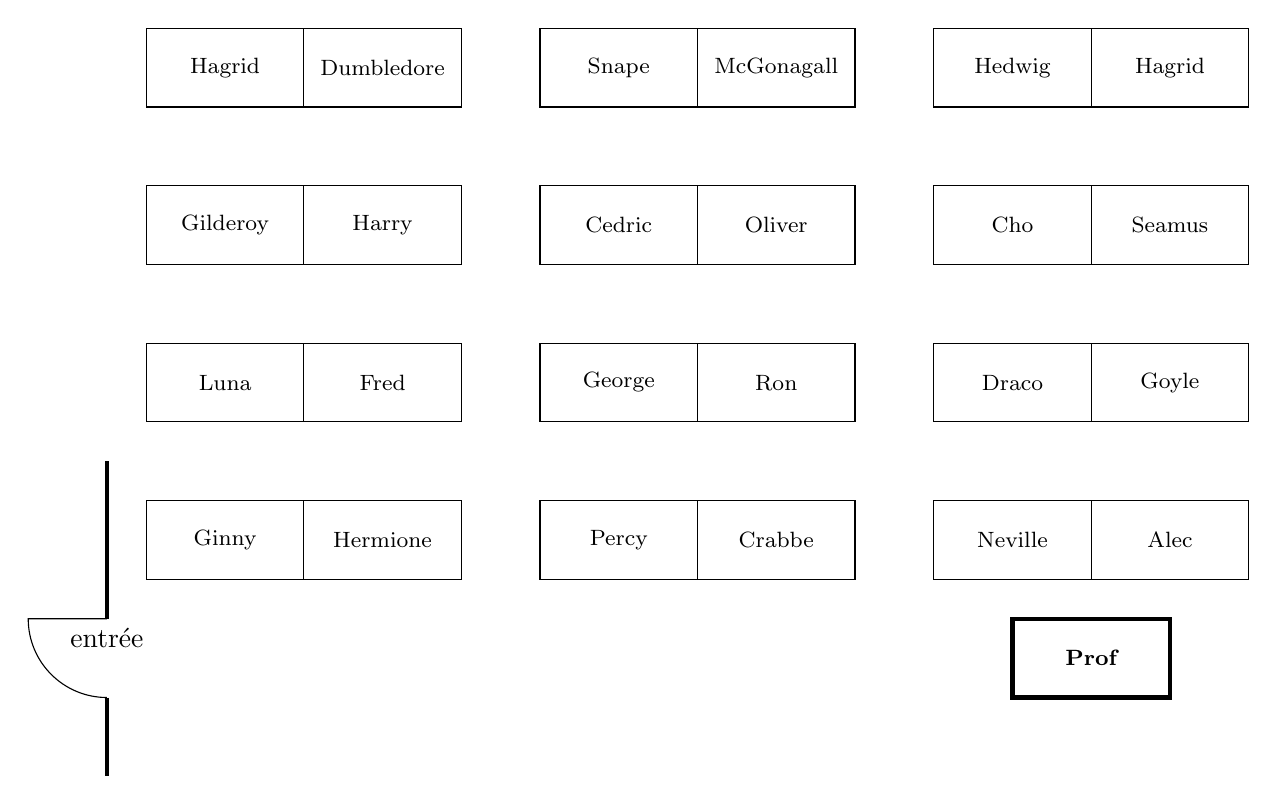
\begin{tikzpicture}

% Students
\node[desk] at (0,0) {Ginny};
\node[desk] at (2,0) {Hermione};
\node[desk] at (5,0) {Percy};
\node[desk] at (7,0) {Crabbe};
\node[desk] at (10,0) {Neville};
\node[desk] at (12,0) {Alec};
\node[desk] at (0,2) {Luna};
\node[desk] at (2,2) {Fred};
\node[desk] at (5,2) {George};
\node[desk] at (7,2) {Ron};
\node[desk] at (10,2) {Draco};
\node[desk] at (12,2) {Goyle};
\node[desk] at (0,4) {Gilderoy};
\node[desk] at (2,4) {Harry};
\node[desk] at (5,4) {Cedric};
\node[desk] at (7,4) {Oliver};
\node[desk] at (10,4) {Cho};
\node[desk] at (12,4) {Seamus};
\node[desk] at (0,6) {Hagrid};
\node[desk] at (2,6) {Dumbledore};
\node[desk] at (5,6) {Snape};
\node[desk] at (7,6) {McGonagall};
\node[desk] at (10,6) {Hedwig};
\node[desk] at (12,6) {Hagrid};


% Prof
\node[desk, ultra thick] at (11, -1.5) {\bfseries Prof};

% Door
\draw[ultra thick] (-1.5,1) -- (-1.5, -1);
\draw[ultra thick] (-1.5,-2) -- (-1.5, -3);
\draw (-1.5,-2) arc (270:180:1) -- (-1.5,-1) node[below] {entrée};

\end{tikzpicture}
\end{adjustbox}

\caption{Example of a seating plan, created with the Tikz package of \LaTeX} \label{seatingplan}

\end{figure}





\subsubsection{Exam notes}

The individual exam results will be needed in order to calculate the average note for each student for each semester, section \ref{output_notes}. We will also need the weighting associated with each exam, and by including the date of the exam we can check the progression of students, section \ref{output_report}.




\subsection{Explanation of outputs}

\subsubsection{Suggested students for focus} \label{output_focus}

As a student teacher, I found it hard to balance my time equitably among the students in a class. Certain students, perhaps those who were louder or more confident, tended to capture my attention. By keeping a record of my interactions with students, it was possible to estimate an ordering of students by recent interactions, and so indicate students who require teacher \emph{focus} during the next set of teacher-student interactions (probably during the next class).

This \emph{focus} can be very simple: these are the students to whom the teacher addresses the opening questions. These opening questions can revise topics from the last lesson or prepare the students for the ideas to be tackled in this lesson. J. Larkin and H. Pines point out that students who respond positively to an early question are much more likely to volunteer answers later in the class \cite{Larkin05}. They also suggest supporting shy students by announcing the question in advance of the lesson.

\

Let us model the interactions with a given student by simply counting the number of interactions on a given day.

\begin{tcolorbox}
Comments:

01/06/2023 Harry gives conclusion of Pythag \\
01/06/2023 Harry, Ron correct calc litt \\
04/06/2023 Ron calculates angles in triangle \\
08/06/2023 Harry calculates hypotenuse
\end{tcolorbox}
We define a function $f_H : \mbox{Dates} \to \mathbb{N}$ to count the interactions with Harry
$$ f_{H}(d) = \left\{ \begin{matrix} 2 &  \mbox{if} & d=\mbox{01/06/2023} \\ 1 & \mbox{if} & d=\mbox{08/06/2023}  \\ 0 && \mbox{otherwise.} \end{matrix} \right. $$
and a corresponding function $f_R$ for the interactions with Ron
$$ f_{R}(d) = \left\{ \begin{matrix} 1 &  \mbox{if} & d=\mbox{01/06/2023}  \\ 1 &  \mbox{if} & d=\mbox{04/06/2023}  \\  0 && \mbox{otherwise.} \end{matrix} \right. $$

On a given date $t$ we would like to create a weight operator, $W_t$, which would map these functions to a real number. This operator should measure the number of recent interactions, giving more weight if there have been more interactions. For example, Harry has had more interactions than Ron and so we expect $W_t(f_H) > W_t(f_R)$.

Consider calculating the students for focus just before the holidays or just after the holidays. Assuming the list of comments has not changed, then ideally the \textbf{ordering} of the students by weight would not change. Thus the students for focus should not be dependant on when the algorithm was run. A straightforward property with this behaviour is that all weights change by the same constant. In probability, this is called the \emph{memoryless} property \cite{Norr98} and implies an exponential weighting of the counts:
$$ W_t(f) = \sum_{d \in \mathcal{D}} f(d) \, e^{k(d-t)} $$
where we sum over all dates\footnote{As the number of comments is finite this is really a finite sum.}  and $k>0$ is a constant. Then recalculating the weights after $n$ days gives
$$W_{t+n}(f) = \sum_{d \in \mathcal{D}} f(d) \, e^{k(d-(t+n))} =  e^{-kn} \cdot \sum_{d \in \mathcal{D}} f(d) \, e^{k(d-t)} = e^{-kn} \cdot  W_t(f),$$
so all weights are rescaled by $e^{-kn}$ which does not depend on $f$.

To pick the constant $k$, consider the desired relative weighting between a student to whom we made a comment yesterday, and another who received two comments quite a while ago (but two comments on the same day). How much time should pass in order that both students receive the same weight? Completely subjectively, I assume one week should pass, which gives
$$1 e^{0k} = 2 e^{-7k} \Rightarrow k = \frac{1}{7} \ln {2}  \approx 0.1.$$ 

Ideally negative interactions should \textbf{not} be counted in this weighting; otherwise "difficult" students would be unlikely to ever be chosen for positive interactions.

\subsubsection{Suggested seating plans}

Most classes have 24 students arranged in 12 pairs, with the 12 pairs at desks arranged in 3 columns by 4 rows, see figure \ref{seatingplan} on page \pageref{seatingplan}. There are two obvious seating arrangements : using the ordering from the class list\footnote{The class list is alphabetic on surname. However, due to data privacy concerns the system does not have access to the surname: it only has the email username, see section \ref{dataprivacy}. The alphabetic ordering of the usernames is not necessarily the same as the alphabetic ordering of the fullnames. To avoid this problem I use the class list ordering directly rather than the usernames.} or using a random seating plan. For testing and repeatability it is much easier to use a deterministic algorithm, and so I have preferred using the class list as a default seating plan.

As the year progresses we have more information about the students: pairs that work well together, students who work at similar speeds, students which have different strengths. Could we use the student comments and the exam results to suggest seating plans suited to particular lessons?

\subsubsection{Average notes for the semester} \label{output_notes}

The notes in Genevan institutions range between 1.5 and 6.0. The average note for the semester is a weighted sum of the individual notes of the marked exams of the semester. The individual notes are rounded to the nearest half, whereas the \emph{semestriel} notes are rounded to the nearest tenth. Mathematically, 
$$ n_s = R_{0.1} \Bigg(\frac{\sum_{i \in \mathcal{I}_s} \, w_i \cdot n_i }{\sum_{i \in \mathcal{I}_s} \, w_i}\Bigg)$$
where the index runs over the marked exams of the semester, and $R_s$ is the function that rounds to the nearest multiple of $s$.

It is worth pointing out that the rounding function is \emph{not} continuous. While this is obvious, it can make the semestriel note surprisingly sensitive to small changes in individual exam notes. This also true for the end of year note, which is the \textbf{rounded} average of the semestriel notes:
$$n_y = R_{0.1} \Bigg( \frac{n_{s_1} + n_{s_2}}{2} \Bigg).$$
In general the pass mark is 4.0, and the rounding functions are a big advantage for weak students. Consider a concrete example, where before rounding a student receives $3.85$ for the first semester and $3.95$ for the second. Then the final end of year note is
$$n_y = R_{0.1}  \Bigg( \frac{R_{0.1}(3.85) +R_{0.1}(3.95)}{2} \Bigg) = R_{0.1} \Bigg( \frac{3.9 + 4.0}{2} \Bigg) = R_{0.1}(3.95) = 4.0$$
and the student passes! Fingers crossed this also applies to Master's theses.

\

I would like the system to calculate the semestriel and end of year notes for each student.

\subsubsection{Individual student reports} \label{output_report}

It is often useful to have a quick overview of an individual student's progress. Perhaps beforehand, while planning which students will tackle which activities, or afterwards, when analysing the efficacy of a sequence of lessons. More concretely, such an overview would be very useful when meeting parents, when giving notes, and when asked to comment on their progress in the \emph{conseils de classes} at the end of each semester.

Information that would be useful would be the student name, their given name, the class, a list of the comments concerning this student, their exam notes over time, and a graphical visualisation of their progress. Roughly, the overview would include an A4 page per student which looks something like this:

\begin{center}
\begin{tcolorbox}

harry.pttr \hfill \textbf{Harry} \hfill 1ma1df01

\

\small{
01/06/2023 Harry gives conclusion of Pythag \\
01/06/2023 Harry, Ron correct calc litt \\
08/06/2023 Harry calculates hypotenuse
}

\vspace{10mm}

\begin{center}
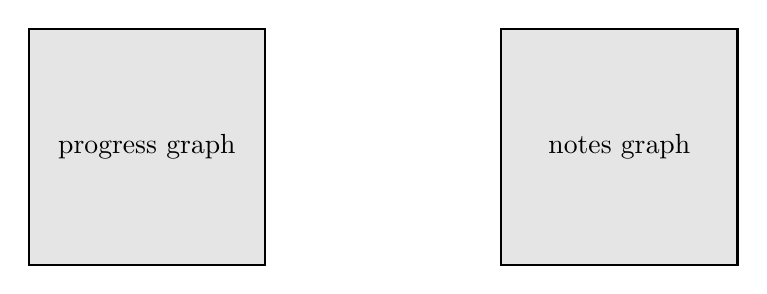
\begin{tikzpicture}

\draw[thick, fill=black!10!white] (0,0) rectangle (3,3) node[pos=0.5] {progress graph};
\draw[thick, fill=black!10!white] (6,0) rectangle (9,3) node[pos=0.5] {notes graph};

\end{tikzpicture}
\end{center}

\end{tcolorbox}
\end{center}


\subsection{Implied structure of backend}

By "backend" I mean the data access layer of the system. By connecting the inputs and outputs we can assess what intermediate processing will be required, and what functionality can be shared. The schematic in figure \ref{dataflowdiagram}, on page \pageref{dataflowdiagram}, is a \emph{Data Flow Diagram} for the TAT system. I have used the Yourdon-Coad notation where the processes (functions) are circles and data is represented by rectangles. Flow of control (transfer of information) is represented by arrows, see \cite{Coad91}.

\begin{figure}[h] 
\begin{center}
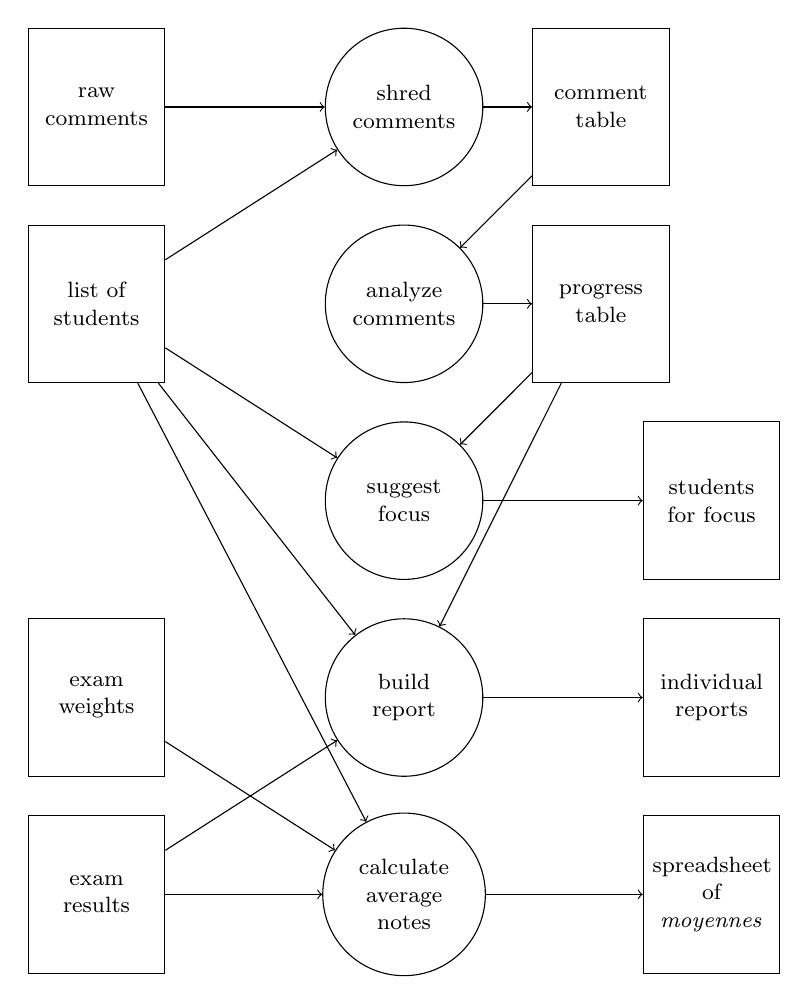
\begin{tikzpicture}[node distance=25mm, every node/.style={draw, text centered, minimum height=20mm, align=center, text width=15mm, font=\fontsize{8}{10}\selectfont}]

\def\datagapmm{40}

\def\function{circle}
\def\datastore{rectangle}
  % Nodes
  \node (comments) [\datastore]{raw comments};
  \node (students) [below of=comments, \datastore] {list of students};
  \node (shred) [right of=comments, xshift=\datagapmm, \function] {shred comments};
  \node (comment_table) [right of=shred, \datastore] {comment table};
  \node (analyze) [below of=shred, \function] {analyze comments};
  \node (progress) [below of=comment_table, \datastore] {progress table};

  % Arrows
  \draw[->] (students) -- (shred);
  \draw[->] (comments) -- (shred);
  \draw[->] (shred) -- (comment_table);
  \draw[->] (comment_table) -- (analyze);
  \draw[->] (analyze) -- (progress);
  
  % Second row
  \node (suggest) [below of=shred, yshift=-25mm, \function] {suggest focus};
  \node (focus) [right of=suggest, xshift=\datagapmm, \datastore] {students for focus};
  \node (build) [below of=suggest, \function] {build report};
  \node (report) [right of=build, xshift=\datagapmm, \datastore] {individual reports};

  \draw[->] (progress) -- (suggest);
  \draw[->] (suggest) -- (focus);
  \draw[->] (progress) -- (build);
  \draw[->] (build) -- (report);
  
  % Third row
  \node (average) [below of=build, \function] {calculate average notes};
  \node (results) [left of=average, xshift=-\datagapmm, \datastore] {exam results};
  \node (weights) [above of=results, \datastore] {exam weights};
  \node (spreadsheet) [right of=average, xshift=\datagapmm, \datastore] {spreadsheet of \emph{moyennes}};
  
  \draw[->] (results) -- (average);
  \draw[->] (weights) -- (average);
  \draw[->] (average) -- (spreadsheet);

  \draw[->] (students) -- (suggest);
  \draw[->] (students) -- (build);
  \draw[->] (students) -- (average);
  \draw[->] (results) -- (build);

\end{tikzpicture}

\end{center}
\caption{Data flow diagram for the backend of the TAT system.} \label{dataflowdiagram}
\end{figure}

The data flow diagram in figure \ref{dataflowdiagram}, on page \pageref{dataflowdiagram}, is a very high-level description of a possible system. To make concrete decisions about how to implement the TAT system it will help to define the expected inputs and outputs. In this section I will outline a basic backend based on files.  An implementation based on files is simpler and quicker, and so more suited for a master's project, but in the future I would expect the backend to handle updates via ACID database queries. I will briefly explain the advantages of databases over files in subsection \ref{db}. I will finish this section by touching on the data privacy laws that apply in Geneva; in particular the system will use only a minimum amount of personal data.

\subsubsection{The list of students}
The \textbf{list of students} is a list of students in each class. I will use a text file for each class, storing a list of user-ids for each student. For example, for the class 1in1dfb01 I would create a textfile called "1in1dfb01.txt":
\begin{tcolorbox}[title = 1in1dfb01.txt]
\texttt{harry.pttr\\ronald.wsly\\marie.cr\\richard.fynmn}
\end{tcolorbox}
This also seems a pertinent place to store the given name of each student. Currently the user-id starts with the first name of the student followed by a fullstop followed by (roughly) the consonants of the surname, 
\begin{center}
\texttt{user\_id = firstname + "." + consonants(surname).}
\end{center}
A regular expression of the form \texttt{\textasciicircum
[a-z\textbackslash-]+} strips the student's first name from their user-id. In Python, we use the \texttt{re} package, for example
\begin{center}
\texttt{firstname = re.search(r"\textasciicircum[a-z\textbackslash-]+", user\_id).group(0).capitalize()}
\end{center}
Applying this function to the students above would yield
\begin{center}
\texttt{["Harry", "Ronald", "Marie", "Richard"]}
\end{center}

However, there are two issues with assuming that this function will always yield the given name of a student. Firstly, we do not control how the user-ids are created, and so we cannot guarantee that this function will work in the future. Secondly, a student might want to be called by a different name (for example their second name). 

I decided to add an optional comma-separated second item which designates the given name of a student in a class: this will be the name shown on the seating plan. For example, if Ronald Weasley wished to be called "Ron" and Richard Feynman preferred "Dick", then the file for the class list would be 
\begin{tcolorbox}[title = 1in1dfb01.txt]
\texttt{harry.pttr\\ronald.wsly, Ron\\marie.cr\\richard.fynmn, Dick}
\end{tcolorbox}

\subsubsection{Raw comments}
The \textbf{raw comments} was originally stored in a text file designed to be read and updated by the teacher. For this project, I have used the same design. A comment is written on a new line in the file, prefaced with a "+" or "-" depending on whether the comment is positive or negative. Then I include a list of students, followed by a comment.\footnote{The text in the comment can handle \LaTeX{} commands}

Examples of positive comments: \\
\texttt{+Harry gives conclusion of Pythag} \\
\texttt{+Harry, Ron correct calc litt for \$(a+b)\textasciicircum2\$}

\

Examples of negative comments: \\
\texttt{-Harry moaning about scar} \\
\texttt{-Harry, Ron chatting}

Before lines of comments there must be a line with the name of the class and, independently, the date. So a valid state for the comments file might be something like the following
\begin{tcolorbox}[title = comments\_file\_v0.1.txt]
\texttt{01Apr2023\\1indfb01\\+Harry gives conclusion of Pythag\\+Harry, Ron correct calc litt for \$(a+b)\textasciicircum2\$\\\\2indfb01\\+George TN for Djikstra \\\\02Apr2023\\1indfb01\\-Ron DNF\\+Harry, Ron TN for Pythagoras}
\end{tcolorbox}
(Note that the vertical spaces are optional and aid human readability.)

(TN is my shorthand for \emph{"l'élève explique au tableau noir"}.)


Given that this is a first implementation, but that nevertheless we want an efficient backend, we can improve the parsing of this file by demanding that the first character in each line defines the information that this line will contain:

\begin{itemize}
\item "+" or "-" will be followed by a comma separated list of students and a comment.
\item "d" will be followed by a date in "ddMMMyyyy" format.
\item "c" will be be followed by a class name.
\end{itemize}

\begin{tcolorbox}[title = comments\_file\_v1.1.txt]
\texttt{d01Apr2023\\c1indfb01\\+Harry gives conclusion of Pythag\\+Harry, Ron correct calc litt for \$(a+b)\textasciicircum2\$\\\\c2indfb01\\+George TN for Djikstra \\\\ d02Apr2023\\c1indfb01\\-Ron DNF\\+Harry, Ron TN for Pythagoras}
\end{tcolorbox}

\subsubsection{Comment table}

The \textbf{comment table} is a pandas data frame\footnote{\texttt{https://pandas.pydata.org/docs/reference/api/pandas.DataFrame.html}} created from the raw comments. The \emph{shred comments} functions read the raw comments from top to bottom, scraping the information in a comment along with the associated student, date, the course name, and the sentiment (whether the comment is positive or negative). A comment in the raw comments file can concern multiple students, so if necessary a line in the data frame is duplicated for each individual student. An example is given on page \pageref{comments_table}, restricting to the columns "Student", "Date", "Course", "Info" and "Sentiment".

\begin{tcolorbox}
NB: I had hoped that the TAT system would also keep track of missed homeworks (\emph{devoirs non-fait} in French, hence "DNF" in the comments). I have decided to punish students with a electronic \emph{renvoi} for every second homework missed. Of course, it is quite a lot of work to track which students have missed a second homework. The TAT system can easily count the DNFs through time which eliminates this bureaucracy (it also avoids mistakes and so is fairer.) The counting of DNFs is implemented in the backend but not yet wired up in the GUI, and so I do not mention it elsewhere in this thesis.
\end{tcolorbox}

\begin{landscape}

\begin{tcolorbox}[title = comments\_file\_v1.1.txt]
\texttt{d01Apr2023\\c1indfb01\\+Harry gives conclusion of Pythag\\+Harry, Ron correct calc litt for \$(a+b)\textasciicircum2\$\\\\c2indfb01\\+George TN for Djikstra \\\\ d02Apr2023\\c1indfb01\\-Ron DNF\\+Harry, Ron TN for Pythagoras}
\end{tcolorbox}


\begin{tcolorbox}[title = comments\_table\_DataFrame $\subset$ progress\_table\_DataFrame] \label{comments_table}

\begin{tabular}{|l|l|l|l|l||l|l|}
\hline
\textbf{Student} & \textbf{Date} & \textbf{Course} & \textbf{Info}                                                               & \textbf{Sentiment} & \textbf{Weight} & \textbf{Progress} \\ \hline
harry.pttr       & 01Apr2023     & 1indfb01        & +Harry gives conclusion of Pythag                                           & 1                  & 0.9             & 1                 \\ \hline
harry.pttr       & 01Apr2023     & 1indfb01        & +Harry, Ron correct calc litt for $(a+b)^2$ & 1                  & 0.9             & 2                 \\ \hline
ronald.wsl       & 01Apr2023     & 1indfb01        & +Harry, Ron correct calc litt for $(a+b)^2$ & 1                  & 0.9             & 1                 \\ \hline
george.wsl       & 01Apr2023     & 2indfb01        & +George TN for Djikstra                                                     & 1                  & 0.9             & 1                 \\ \hline
ronald.wsl       & 02Apr2023     & 1indfb01        & -Ron DNF                                                                    & -1                 & 0.0             & 0                 \\ \hline
harry.pttr       & 02Apr2023     & 1indfb01        & +Harry, Ron TN for Pythagoras                                                & 1                  & 1.0             & 3                 \\ \hline
ronald.wsl       & 02Apr2023     & 1indfb01        & +Harry, Ron TN for Pythagoras                                                & 1                  & 1.0             & 1                 \\ \hline
\end{tabular}
\end{tcolorbox}

\end{landscape}

\subsubsection{Progress table}
In the \textbf{comments table} the columns were "Student", "Date", "Course", "Info" and "Sentiment". To these columns we adjoin the "Weight" and "Progress" columns to create \textbf{progress table}, which (like the comments table) is also implemented as a pandas DataFrame. See the example on page \pageref{comments_table}.

The \emph{weight} of a positive comment is a memoryless function of the time duration between now and the date associated with the comment, see subsection \ref{output_focus} on page \pageref{output_focus}:
$$ \mathrm{weight} = e^{-kd} $$
where $d$ is the age of the comment in calendar days and $k = 0.1$ is a constant. For example, the weight of a comment made today is $e^{-0.1 \cdot 0} = 1$ while the weight of a comment made yesterday is $e^{-0.1 \cdot 1} \approx 0.9$. Comments with a negative sentiment have a weight of 0 (forgive and forget).

The \emph{progress} is the running cumulative sum of sentiments filtered on that student in that class. If we filter the progress table on \texttt{harry.ptter} in course \texttt{1indfb01} then we see

\

{\footnotesize
\hspace{-6mm}
\begin{tabular}{|l|l|l|l|l|}
\hline
\textbf{Date} & \textbf{Info}                                                               & \textbf{Sentiment} & \textbf{Weight} & \textbf{Progress} \\ \hline
01Apr2023     & +Harry gives conclusion of Pythag                                           & 1                  & 0.9             & 1                 \\ \hline
01Apr2023     & +Harry, Ron correct calc litt for $(a+b)^2$ & 1                  & 0.9             & 2                 \\ \hline
02Apr2023     & +Harry, Ron TN for Pythagore                                                & 1                  & 1.0             & 3                 \\ \hline
\end{tabular}
}


\subsubsection{Students for focus}
We sort the set of students in a given course to return a list of \textbf{students for focus}, a list ordered in increasing need for teacher-student interactions. This "need" is approximated by a function of the distribution of the comments over time, as explained in subsection \ref{output_focus} on page \pageref{output_focus}. In practice, it is simply the sum of the weights in the progress table. Referring to the example on page \pageref{comments_table}, the sum of weights for the students in class \texttt{1indfb01} is
\begin{center}
\texttt{\{"harry.pttr": 2.8, "ronald.wsl": 1.9\}}.
\end{center}
So as a list ordered on increasing weight, the students for focus would be
\begin{center}
\texttt{["ronald.wsl", "harry.pttr"]}.
\end{center}
Of course, other students in this course have a default weight of zero if there are currently no comments associated to them. So if the course also included \texttt{"hermione.grngr"} then the ordered list of students for focus would be
\begin{center}
\texttt{["hermione.grngr", "ronald.wsl", "harry.pttr"]}.
\end{center}

\subsubsection{Report}
The \textbf{report} is a pdf document containing an A4 page per student. On each page we have the student-id, the student's given name, the course, and a list of comments associated with this student. The TAT system first creates a text-based .tex document, and then calls a system function which executes pdflatex\footnote{\texttt{https://www.tug.org/applications/pdftex/}} to typeset the report as a .pdf document.

\subsubsection{Spreadsheet of moyennes}
The TAT system can shred spreadsheets of individual exams to create a table with the exam name, exam date, course, student-ids and associated notes. It then creates a \textbf{spreadsheet of moyennes} with a worksheet per course and a table of notes with the exams as columns and the student-ids as rows.

So far, the description above explains how a spreadsheet of static data is created (albeit static data collated in a useful single file). The TAT system goes further, automatically creating a table of cells containing formulae (rather than static data) which calculate the student \emph{moyennes} for the provisional notes (NIPs), the first semester notes (S1), the second semester notes (S2) and the implied end of year note (EOY). This allows the teacher to fill-in or correct individual exams and see the effect on the notes to be officially declared. Further, by leaving rows for the individual exam weights the teacher has the flexibility to specify which exams are noted and which are formative, which exams count double, as well as choosing the weight of the semestriel exams.

The algebra for the calculation of the notes was given in subsection \ref{output_notes}, on page \pageref{output_notes}. The equivalent spreadsheet formulae are 
\begin{itemize}
\item \texttt{"RAWNOTE=SUMPRODUCT(EXAMWEIGHTS, EXAMNOTES)/SUM(EXAMWEIGHTS)},
\item \texttt{"NOTE\_Sx=ROUND(RAWNOTE*10)/10"}, and
\item \texttt{"NOTE\_EOY=ROUND(AVERAGE(NOTE\_S1;NOTE\_S2)*10)/10"}.
\end{itemize}

I also made the TAT system create the workbook with conditional formatting applied to the cells, so that notes less than the passing mark of 4.0 are flagged in red. To handle missing notes (for example, when students were absent), I use a default value of -100 as I did not want to expose non-scientific users to the joys of \texttt{NaN}, the representation of the idea of "Not a Number". The value of -100 is sufficiently negative to cause obvious problems throughout the calculations.

\subsubsection{Exam results}
In order to shred individual exams that TAT system assumes that the notes are stored in spreadsheets named with the convention \texttt{EXAMDATE\_EXAMNAME\_Notes} with extension either \texttt{.ods}, \texttt{.xls} or \texttt{.xlsx}. The files for a single course should be grouped together in a subdirectory with the same name as the course name. Each spreadsheet must contain a cell in the first column containing the keyword "Student", followed by a column of student-ids. There should be a cell in the first row containing the keyword "Note", and the notes are in the corresponding intersection of the student-id row and the note column. These are notes for an individual exam, and so should be rounded to the nearest multiple of 0.5.\footnote{Individual exam notes are given to the nearest half except in very special cases. One such exception is for controlled exams with an external jury: where the teacher and the jury agree to disagree, the exam note is the average (rounded to the nearest tenth) of the two notes (rounded to the nearest half).}

So an example for an exam filename might \texttt{20Apr2020\_ExampleExam\_Notes.ods} found in the directory \texttt{.\textbackslash1indfb01}.


\subsubsection{Databases} \label{db}
In the Genevan \emph{plan d'études} one third of the second year is devoted to databases (ten out of thirty contact hours). This project would have been excellent opportunity for me to practice planning, creating, updating and querying tables programmatically: the course lists, the comment table and the progress table lend themselves naturally to being stored and treated as tables in a database (indeed, that's why I named them as tables).

Using a database has a number of advantages over a system based on flat files, including:
\begin{enumerate}
\item handling scalability and concurrency, 
\item data organisation and structure,
\item providing automated backup and recovery programs,
\item offering user authentication and enhanced data security, as well as
\item data consistency based on ACID transactions.
\end{enumerate}
The first four reasons are less important for small, individual projects such as this masters. The last reason, however, would have been useful: ACID stands for Atomicity, Consistency, Isolation, and Durability. Consistency promises that the databases is always in a valid state, even if the system crashes during an update. The TAT system does not make this promise with flat text files: if the system only adds the first few letters of a course name in the raw comments file, for example, the TAT system will not be able to restart without a manual intervention.

\begin{tcolorbox}[title = comments\_file\_BROKEN.txt]
\texttt{d01Apr2023\\c1indfb01\\+Harry gives conclusion of Pythag\\+Harry, Ron correct calc litt for \$(a+b)\textasciicircum2\$\\\\c2ind}
\end{tcolorbox}

In spite of these advantages I decided to leave the TAT system based on flat files. First, there is the non-negligible cost and risk of migration (although the risk is minimised with a good testing framework, see \ref{tdd} on page \pageref{tdd}). Second, for novice users the readable files make adjustments much easier while the GUI is not fully refined. Thirdly, as explained in the next section, by basing the system on files which could be reasonably expected to be found on an average teachers' computer, we are still within the remit of current data privacy recommendations. If the system began storing the data in a novel way then it would possibly need to be reassessed by the \emph{Préposé cantonal à la protection des données et à la transparence} (PPDT)\footnote{\texttt{https://www.ge.ch/organisation/protection-donnees-transparence}}.

\subsubsection{Data privacy} \label{dataprivacy}

In the course "Security and Confidentiality" given by Linus Gasser at EPFL, all GymInf students have studied the most relevant laws governing IT systems. In Geneva, for example, we must be follow the Swiss "Federal Act on Data Protection"\footnote{\texttt{https://www.fedlex.admin.ch/eli/cc/1993/1945\_1945\_1945/en}}, called \textbf{LIPAD} by the Genevan authorities, and we should also check that we do not have to follow the much more stringent European "General Data Protection Regulation"\footnote{https://eur-lex.europa.eu/legal-content/EN/TXT/?uri=CELEX\%3A02016R0679-20160504}, called the \textbf{GDPR}, which is extraterritorial.

Luckily, public schools in the Genevan canton do not need to follow the GDPR. This was decided by the \emph{Préposé cantonal à la protection des données et à la transparence} (PPDT)\footnote{\texttt{https://www.ge.ch/organisation/protection-donnees-transparence}} in 2018:
\begin{center} 
\emph{"Ainsi, ne sont en principe pas soumises au RGPD les situations suivantes... L’instruction publique accueille des élèves qui résident et/ou ont la nationalité d’un Etat membre de l’UE, sans avoir fait de promotion sur le territoire de l’UE."}\cite[p. 3]{PPDT18}
\end{center}
In the same document the PPDT reminds us that we should follow LIPAD with respect to sensitive personal data:
\begin{center} 
\emph{"Les institutions publiques genevoises sont soumises à la LIPAD, s'agissant du traitement des données personnelles (art. 3 LIPAD). Elles doivent donc respecter les dispositions prévues par cette loi dans tout traitement de données personnelles."}\cite[p. 1]{PPDT18}
\end{center}
The LIPAD defines sensitive personal data as
\begin{enumerate}
\item religious, ideological, political or trade union-related views or activities,
\item health, the intimate sphere or the racial origin,
\item social security measures,
\item administrative or criminal proceedings and sanctions; and also
\item a \emph{personality profile}: a collection of data that permits an assessment of essential characteristics of the personality of a natural person.
\end{enumerate}

As implemented, the TAT system uses the same information that an average teacher would already be storing about their students in order to carry out their duties. Therefore the TAT system stays within the current framework and findings. However, if we collated much larger amounts of student information in a single database it might be argued that this personal data constituted a \emph{personality profile}, which would be covered by the LIPAD. To avoid having to check this during the masters project, I decided not to implement a database and instead make use of existing files.






\section{Choice of programming language} \label{language}

\subsection{Previous personal experience}

I have experience programming in a number of languages : I used \textbf{Basic} and a bit of \textbf{assembler} as a child, then \textbf{Delphi} (Visual Pascal) as a teenager, next \textbf{C++} as a grad student, and then I used \textbf{Java} and \textbf{Matlab} extensively when I worked in industry. I tried \textbf{Scala}, \textbf{Clojure} and \textbf{Julia} during my years transitioning to teaching, and more recently during my GymInf studies I have also had to learn \textbf{Python} and \textbf{Prolog}.

In general, apart from Prolog, these languages feel quite similar. Some are more weighted towards object-oriented programming (Delphi, Java and Scala) but in general the virtual machine can be modelled as storing the program as a text file and executing the instructions line by line. Variables are declared and assigned values, and expressions are evaluated using iterative rules. Except for Basic and Assembler, which still allow Djikstra's nemesis the \texttt{GOTO} command, the virtual machine has control of the general flow of the execution using \emph{functions} or \emph{events} (the latter are in some sense just functions owned or controlled by objects). If we ignore naughty tricks, the programmer can only use switch statements, \texttt{if-elif-else}, \texttt{switch}, or \texttt{case}, to adjust the execution path at a very local level.

The other distinction between the languages is whether or not they are \emph{functional}. Functional languages do not allow the redefinition of a variable, such as Prolog, Clojure and Scala. 

I considered the following factors when choosing the language for my project:
\begin{itemize}
\item my current proficiency,
\item my interest for improving my proficiency,
\item ease for finding solutions to coding problems,
\item readability of the code,
\item maintainability of the code, and
\item future applications of improved coding abilities.
\end{itemize}

There are other factors which did not affect my decision at the start of coding : for example, creating the GUI (graphical user interface), deployability of the code, the speed and reactivity of the program, or whether the code would be scalable. I will comment on these oversights in the conclusion.

Alongside \textbf{Scala} (syntactic sugar over Java with a functional feel) and \textbf{Julia} (Matlab maths functionality built directly on C++), the other \emph{new} languages I considered using were \textbf{Swift}, \textbf{Clojure} and \textbf{Rust}.

\subsection{Python} \label{python}
At Collège Rousseau, where I teach, we decided to teach the students Python. This was a difficult decision, with each language having advantages and disadvantages. Like the vast majority of Secondary II schools in Switzerland, we decided that the low barrier to entry, the wide use of Python in industry, the teachers' current abilities, the availability of packages, the large support community, and the focus on readability narrowly outweighed the use of weak (duck) typing with beginners.

The teacher is expected to have a strong background in the coding language being taught :
\begin{itemize}
\item for the pedagogical benefits of "live coding", modelling how to create code for the students to discuss and learn from \cite{Raj2018}, 
\item creating well written code for students to study,
\item for ease of marking and correcting (lots of) student code,
\item for spotting mistakes in student code during class time, in order to suggest hints,
\item for recognising bad coding practices and explaining to students the potential pitfalls and how to avoid them, and
\item for understanding error messages.
\end{itemize}







\section{Test-Driven Development} \label{tdd}
The process of developing complex IT systems involves various stages, from understanding client requirements to delivering and maintaining the final product. Traditionally, software development followed the waterfall method \cite[p. 53]{Amman16}, where each phase was executed sequentially: 
\begin{itemize}
\item requirements  analysis, 
\item design, 
\item implementation, 
\item testing, and 
\item deployment. 
\end{itemize}
In their 2016 book, Ammann and Offutt speculate that the waterfall method originated with software development for large military projects. Here software was expected to have a long lifetime with no maintenance \cite[p. 96]{Amman16}. However, in industry this approach had several drawbacks, such as a long development cycle and limited client involvement until the final stages.  

Reviews with the clients at a late stage of the development cycle led to misunderstandings and mismatches between the final product and client expectations. This resulted in costly redesigns that would have been cheaper if they had been identified earlier in the process, or even projects being dropped altogether. In 2004, a study showed that 45\% of IT projects in the US failed to meet user requirements \cite[p. 88]{LX10}. In this section I explore how industry practitioners have tried to adapt the waterfall process and the introduction of test-driven development.

\subsection{Reducing the distance between clients and developers}
As a response to costly overruns the \textbf{Agile} methodologies emerged in the early 2000s, emphasising iterative development and client collaboration \cite{Anaya18, Beck03}. The adoption of Agile methodologies aimed to bridge the gap between clients and developers throughout the process. Agile principles emphasise frequent communication, iterative development, and the delivery of working software in short cycles known as \emph{sprints}. I would argue that autonomous teams of developers were encouraged to take control of the waterfall method themselves, but on a timescale of weeks rather than years. This approach allowed clients to see progress regularly, provide feedback, and steer the development process in the right direction. 

Note that even with Agile principles it is still difficult to ensure that the delivered software precisely meets the client's needs. Further, as G. Lee and W. Xia pointed out in 2010, much of the alleged advantages of Agile development are anecdotal rather than scientifically proven \cite{LX10}. They found that there is a difference between being able to quickly respond to a particular change in user requirement (response efficiency), compared to being able to respond to as many changes as possible (response extensiveness). Encouragingly, with this distinction they did find evidence that agile teams with more autonomy had greater response efficiency, and that response efficiency positively effects all measures of project success \cite[pp. 97-98]{LX10}.


\subsection{Testing} \label{testing}
The shorter sprints and early involvement of clients may have led to developers becoming used to the idea of shipping beta versions of their software, rather than aiming for a final version. Another problem independently emerging in the 1990s was the increasing cost of \emph{maintaining} delivered systems. For these reasons the \textbf{testing} of software evolved.

Ammann and Offutt state that \emph{"faults in software are design mistakes\ldots they exist as a result of a decision by a human"} \cite[p. 29]{Amman16}. Since humans make mistakes, we must assume that software contains bugs. This in turn means we cannot prove that code is correct.\footnote{This is a long way from E. Djikstra's ideal of proving correctness of code, but the complexity of even moderately sized programs rules this out in practice.} So why do we test code? Ammann and Offutt identify five levels of increasing understanding to this question:
\begin{enumerate}
\item There is no difference between testing and debugging.
\item The purpose of testing is to show correctness.
\item The purpose of testing is to show that the software does not work.
\item The purpose of testing is to reduce the risk of using the software.
\item Testing is a mental discipline that helps all IT professionals develop higher-quality software.
\end{enumerate}

There are different types of testing. \textbf{Unit testing} compares inputs and outputs to check the functions behave as expected in a finite set of situations. Choosing these situations to cover as many interesting use-cases as possible becomes part of mental discipline mentioned above. \textbf{Integration testing} focuses on how different modules interact. \textbf{Regression testing} compares previous outputs against current outputs after a software update. \textbf{User acceptance testing} involves clients evaluating the system to determine if it meets their expectations.

\begin{center}
\emph{While this approach to correctness might strike mathematicians as impoverished, software is built by engineers, and guess what? Engineers are not mathematicians!} \cite[p. 98]{Amman16}
\end{center}

But there is still a problem: once the code is developed, who is doing the testing? If the developers and the testers are different teams, then it is hard to avoid a level 3 mindset (showing that the software does not work). But if the developers test their own code there is a risk of a level 2 mindset (testing shows correctness, which is impossible).

\subsection{TDD: Test-Driven Development}
To avoid these issues altogether and hence promote a level 5 mindset (that testing is a mental discipline which improves coding) K. Beck and his collaborators suggested that the developers should write their own tests \emph{before} they wrote their code \cite{Beck03}. This practice became known as \textbf{test-driven development}, or TDD. To help developers use this counterintuitive practice, there is a simple cycle to follow:
\begin{itemize}
\item \textbf{Red.} Write a failing test for a requirement.
\item \textbf{Green.} As quickly as possible, write code to pass the test.
\item \textbf{Refactor.} Clean the code, removing duplication and renaming functions.
\end{itemize}
Coding is driven by testing.

Let us consider an explicit example from the TAT system: running the application for the first time, when there are no files or folders pre-created. We expect the TAT application to run with no courses listed, ready for the user to add courses (and students), and we also expect that the folder structure is automatically set up to handle the future files. Currently the GUI crashes almost immediately - it does not find the expected \texttt{config.yaml} config file. So let's use TDD to write code to create a default config file. 

\subsubsection{Red}
The desired code lives naturally in the module \texttt{config.py}, but first we write the test in \texttt{tests/config\_test.py}:
\begin{lstlisting}
import config
import os


def test_create_default_cfg_file(tmp_path):
    f = os.path.join(tmp_path, , "config.yaml")
    config.default(f)
    assert os.path.isfile(f)
\end{lstlisting}
Note that \texttt{tmp\_path} is a PyTest fixture which creates a temporary folder for this test: PyTest handles setting up and tearing down the temporary folder. We run the PyTest suite and, of course, the test crashes with \texttt{AttributeError: module 'config' has no attribute 'default'}. However, this is not truly a failing test - the test \textbf{crashed} rather than an assertion failing. We need to write an empty function in \texttt{config.py}:
\begin{lstlisting}
def default(f):
    pass
\end{lstlisting}
Now PyTest fails with an \texttt{AssertionError}, so we have successfully completed the \textbf{Red} part of the cycle.

\subsubsection{Green}
Now we code the function \texttt{default.py}.
\begin{lstlisting}
import os

def default(f):
    open(f, 'w').close
\end{lstlisting}
We run PyTest again and all tests trivially pass. Yay!

\subsubsection{Refactor}
In this case the code is already as simple as possible. \textbf{We're done.} This feels wrong, since we know that we have created an empty file instead of a working config file. But since the tests are passing we are not (yet) forced to write the correct code and so we do not.

\subsubsection{Red}
Now we have the idea, we can try moving a little faster. The new default config file should contain paths to the folder which will hold the exam results. We would like a function which sets up the basic structure, so we start with the \texttt{exams} subdirectory.

\begin{lstlisting}
import config
import os


def test_create_default_cfg_file(tmp_path):
    f = os.path.join(tmp_path, , "config.yaml")
    config.default(f)
    assert os.path.isfile(f)
    
    
def test_basic_structure_from_cfg_file(tmp_path):
    f = os.path.join(tmp_path, "config.yaml")
    exam_dir = os.path.join(tmp_path, "exams")
    config.default(f)
    config.setup_from_cfg_file(f)
    assert os.path.isdir(exam_dir)
\end{lstlisting}

\begin{lstlisting}
def default(f):
    open(f, 'w').close()


def setup_from_cfg_file(f):
    pass
\end{lstlisting}
As well as the test, I've written a placeholder for the new function. PyTest fails with an \texttt{AssertionError}, so we have completed the \textbf{Red} phase.

\subsubsection{Green}
We write a truly horrific bit of code to make the test pass:
\begin{lstlisting}
import os


def default(f):
    open(f, 'w').close()


def setup_from_cfg_file(f):
    os.mkdir(f.replace("config.yaml", "exams"))
\end{lstlisting}
PyTest is happy (even if you are not), so \textbf{Green} is complete.

\subsubsection{Refactor}
You may want to sit down at this point: there is refactoring to be done, but it's not in \texttt{config.py}. We refactor the tests in \texttt{test\_config.py}:
\begin{lstlisting}
import config
import os


def create_cfg_file(path):
    f = os.path.join(path, "config.yaml")
    config.default(f)
    return f


def test_create_default_cfg_file(tmp_path):
    assert os.path.isfile(create_cfg_file(tmp_path))


def test_basic_structure_from_cfg_file(tmp_path):
    f = create_cfg_file(tmp_path)
    config.setup_from_cfg_file(f)
    exam_dir = os.path.join(tmp_path, "exams")
    assert os.path.isdir(exam_dir)
\end{lstlisting}
We rerun the tests to check that the refactoring does not break any of the tests, and the \textbf{Refactor} is done.

\subsubsection{Red}
Before we've tried test-driven development, this feels completely wrong. How can we still have the code \texttt{os.mkdir(f.replace("config.yaml", "exams"))} ? In my opinion, we treat coding as a three-player game : code as succinctly as possible in the Green phase, refactor as much as possible in the Refactor phase, and then try to think of tests which will force the code in the right direction in the Red phase. This leads to the level 5 mindset of subsection \ref{testing}, where \emph{testing is a mental discipline}.

So how could we force the green player to create a real config file, and then use this to create the exam folder specified in this config file? We could change the config file with a new location for the exam folder!
\begin{lstlisting}
import config
import os


def create_cfg_file(path):
    f = os.path.join(path, "config.yaml")
    config.default(f)
    return f


def test_create_default_cfg_file(tmp_path):
    assert os.path.isfile(create_cfg_file(tmp_path))


def test_basic_structure_from_cfg_file(tmp_path):
    f = create_cfg_file(tmp_path)
    config.setup_from_cfg_file(f)
    exam_dir = os.path.join(tmp_path, "exams")
    assert os.path.isdir(exam_dir)


def test_tweak_structure_from_cfg_file(tmp_path):
    f = create_cfg_file(tmp_path)
    cfg = config.load(f)
    exam_dir = os.path.join(tmp_path, "exams2")
    cfg["exam_path"] = exam_dir
    config.setup_from_cfg_file(f)
    assert os.path.isdir(exam_dir)
\end{lstlisting}
Now all hell breaks lose, as \texttt{config.load()} finds an empty yaml file.

\subsubsection{Green}
We will need to create a yaml file with the correct fields otherwise \texttt{config.load()} does not run. And then we need to really use that the value in the field \texttt{exam\_path} when we create the exams directory.
\begin{lstlisting}
import os


def default(f):
    path, _ = os.path.split(f)
    config = {
        "courses": [],
        "courses_path": path,
        "exam_path": os.path.join(path, "exams")
    }
    save(config, f)


def setup_from_cfg_file(f):
    cfg = load(f)
    os.mkdir(cfg["exam_path"])
\end{lstlisting}

\subsubsection{Refactor}
Looking at the tests, it seems odd that we need to load and save the config dictionary. We should return the config dictionary directly, rather than using the filename.

I also refactor the function \texttt{default()}, which is currently storing the information for the default dictionary and also saving it. These roles become \texttt{default\_config()} and \texttt{create\_default()} respectively.
\begin{lstlisting}
import config
import os


def create_cfg_file(path):
    f = os.path.join(path, "config.yaml")
    return config.create_default(f), f


def test_create_default_cfg_file(tmp_path):
    _, f = create_cfg_file(tmp_path)
    assert os.path.isfile(f)


def test_basic_structure_from_cfg_file(tmp_path):
    cfg, _ = create_cfg_file(tmp_path)
    config.setup_from_cfg(cfg)
    exam_dir = os.path.join(tmp_path, "exams")
    assert os.path.isdir(exam_dir)


def test_tweak_structure_from_cfg_file(tmp_path):
    cfg, _ = create_cfg_file(tmp_path)
    exam_dir = os.path.join(tmp_path, "exams2")
    cfg["exam_path"] = exam_dir
    config.setup_from_cfg(cfg)
    assert os.path.isdir(exam_dir)
\end{lstlisting}

\begin{lstlisting}
import os


def default_config(base_path):
    return {
        "courses": [],
        "courses_path": base_path,
        "exam_path": os.path.join(base_path, "exams")
    }


def create_default(f):
    base_path, _ = os.path.split(f)
    config = default_config(base_path)
    save(config, f)
    return config


def setup_from_cfg(cfg):
    os.mkdir(cfg["exam_path"])
\end{lstlisting}

At the point the code feels well-structured. There is a reasonable test coverage, and so I have the confidence to refactor or experiment. I continue cycling through red, green, refactor until the GUI can run from a "cold start".

\

I implemented the backed of the TAT system using test-driven development. Currently I have about 575 lines of code and 350 lines of tests. The tests were written with \textbf{pytest}, which runs all of the tests automatically. I will comment on how I found this in the conclusion, see section \ref{conclusion} on page \pageref{conclusion}.


\section{The graphical user interface} \label{gui}

Initially I had planned to interact with the TAT system using a \emph{Command Line Interface}, updating flat files using a text editor and then calling the Python code from the terminal. To make the system accessible to a wider audience it was suggested that I add a \emph{graphical user interface}, or GUI (pronounced \emph{"gooey"}), over the backend.

In W. Martinez's 2011 article \cite{Mart11} introducing graphical user interfaces the author explains that for most users the GUI is the standard form of human-computer interaction: windows, buttons, drop-down menus, spreadsheets, progress bars, etc. provide a graphical buffer on the screen between the human and the program being executed on the computer. GUIs tend to be \emph{event-based}, driven off user events such as mouse actions and keyboard entry.

In this section I explain how I chose to implement the GUI; both the language and the approach. I then list a few basic principles of GUI design from the literature before outlining the interface I built.

\subsection{Choice of language}

As in subsection \ref{python}, I decided to continue with Python when implementing the GUI. Again the aim was to improve the programming skills I use in class, while gaining experience in areas of computing which offer different directions for my teaching.

Even then, there are many Python packages available for building a GUI. Some packages create familiar "windows": for example \textbf{Tkinter}, \textbf{PyQt}, \textbf{wxPython} and \textbf{PyGTK}. These packages create \emph{widgets} such as buttons, menus, and text editors with standard behaviours. Fitting the widgets into the window as well as handling mouse and keyboard events is done by the package.The widgets can be \emph{"wired up"} to Python functions in the backend. 

The disadvantage with the applications built with these packages is their "look": the GUIs feel old-fashioned which would reduce student interest.

A completely different approach, which is now very popular, is to create an interactive web application. These packages are more diverse than the standard "windows" style packages. There is the pythonic \textbf{JustPy}, lightweight packages such as \textbf{Flask} and \textbf{Remi}, and the full-stack solution \textbf{Django}. These packages can be run locally, serving a webpage which presents the user interface in a navigator, or if hosted on a server then a user can access them from any device with an internet connection. This makes it easier to deploy and share the application with users.

I opted for a third approach: building a GUI from the ground up with \textbf{PyGame} \cite{KK16}. PyGame is a popular Python library for game development, especially 2D games. I have already had a number of students use PyGame in class and the results are almost always impressive: the imagination of the students, their perseverance in the face of difficulties, and the end results. Allowing the students to build their own projects, with more or less scaffolding as required, helps foster internal motivation as explained in the classical literature by R. Viau \cite{Viau94}.

PyGame provides a built-in event queue that collects and manages events such as mouse clicks, keyboard presses, window resizing, etc. This event handling allows developers to create interactive applications that respond to user actions in real-time. As mentioned above GUIs tend to be event-driven and so this is pertinent for GUIs as well as for games.

\

I thought that the TAT system would be a good chance to improve my own PyGame skills.


\subsection{Planning for a positive user experience}
J. Johnson outlines some simple ideas for improved \emph{"UX"}, user experience, in his 2020 book on "GUI Bloopers" \cite{JJo20}. He suggests the user will feel more in control if the design elements and interactions are simple and standardised, feedback is prompt and useful (obvious button clicks, error messages, progress indicators), and actions can easily be undone. Martinez summarises Johnson's ideas into four principles \cite[p. 123]{Mart11}:
\begin{enumerate}
\item ‘Focus on the users and their tasks, not the technology’.
\item ‘Consider function first, presentation later’.
\item ‘Conform to the user’s view of the task: do not make it more complicated’.
\item ‘Promote learning and deliver information, not just data’.
\end{enumerate}

There are strong links to D. Norman's ideas in "The Design of Everyday Things" \cite{Norm13}. Good design should be intuitive and make it easy for users to understand and interact with the objects or systems, which in turn positively influences user behaviour and promotes satisfaction. Norman introduces the concept of \emph{"affordances,"} which refers to the perceived actions that an interface suggests to the user. Clear affordances will guide users on how to use the interface naturally.

So rather than starting with what the backend can do, the design process starts with what the user will want to achieve with the TAT system:
\begin{enumerate}
\item Review and update the list of courses.
\item Edit the list of students in a course.
\item Change the seating plan in a given course.
\item Record a comment for a set of students.
\item Suggest students for next teacher-student focus.
\item Build student reports.
\item Calculate average notes.
\end{enumerate}

\subsection{Views}
A classic GUI structure is to use \emph{views}, different screens designed for different use cases. I based the GUI views on the two phases defined when reviewing the types of actions in the last section: configuration and teaching. I have called the respective views the \textbf{control view} and the \textbf{class view}.

\subsubsection{Control view}

\begin{center}
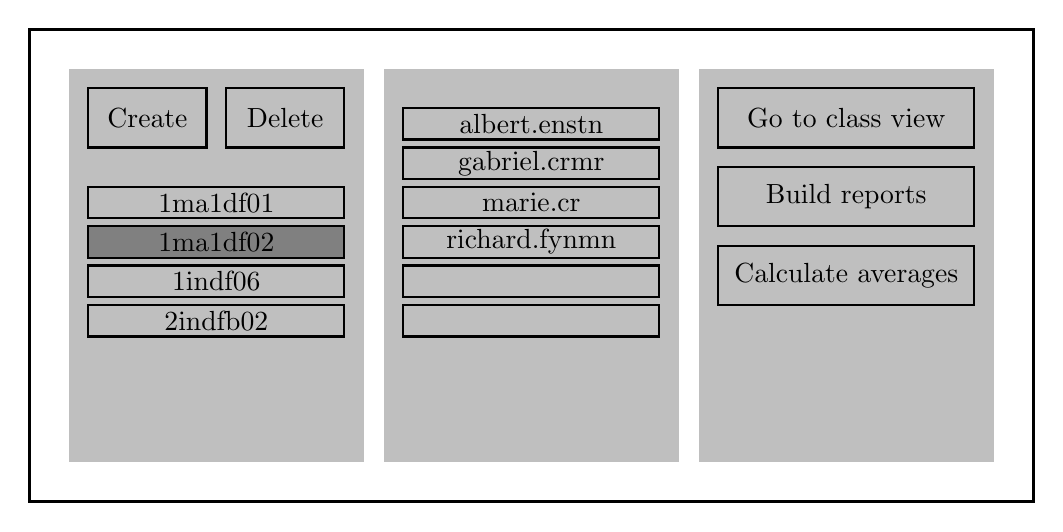
\begin{tikzpicture}

\draw[very thick] (0,0) rectangle (12.75, 6);

\fill[gray!50!white] (0.5, 0.5) rectangle (4.25, 5.5);
\draw[thick] (0.75, 4.5) rectangle (2.25, 5.25) node[pos=0.5] {Create};
\draw[thick] (2.5, 4.5) rectangle (4, 5.25) node[pos=0.5] {Delete};
\draw[thick] (0.75, 3.6) rectangle (4, 4) node[pos=0.5] {1ma1df01};
\draw[fill=gray, thick] (0.75, 3.1) rectangle (4, 3.5) node[pos=0.5] {1ma1df02};
\draw[thick] (0.75, 2.6) rectangle (4, 3) node[pos=0.5] {1indf06};
\draw[thick] (0.75, 2.1) rectangle (4, 2.5) node[pos=0.5] {2indfb02};

\fill[gray!50!white] (4.5, 0.5) rectangle (8.25, 5.5);
\draw[thick] (4.75, 4.6) rectangle (8, 5) node[pos=0.5] {albert.enstn};
\draw[thick] (4.75, 4.1) rectangle (8, 4.5) node[pos=0.5] {gabriel.crmr};
\draw[thick] (4.75, 3.6) rectangle (8, 4) node[pos=0.5] {marie.cr};
\draw[thick] (4.75, 3.1) rectangle (8, 3.5) node[pos=0.5] {richard.fynmn};
\draw[thick] (4.75, 2.6) rectangle (8, 3);
\draw[thick] (4.75, 2.1) rectangle (8, 2.5);

\fill[gray!50!white] (8.5, 0.5) rectangle (12.25, 5.5);
\draw[thick] (8.75, 4.5) rectangle (12, 5.25) node[pos=0.5] {Go to class view};
\draw[thick] (8.75, 3.5) rectangle (12, 4.25) node[pos=0.5] {Build reports};
\draw[thick] (8.75, 2.5) rectangle (12, 3.25) node[pos=0.5] {Calculate averages};


\end{tikzpicture}
\end{center}

Possible events controlled from this view: 
\begin{enumerate}
\item Create a new class.
\item Select the active class.
\item Delete the active class
\item Edit the class list.
\item Pass to the class view of the active class.
\item Build student reports.
\item Calculate average notes.
\end{enumerate}

\subsubsection{Class view}

The class view includes the seating plan, both as a reminder for names and as a visual cue for interactions.

\begin{center}
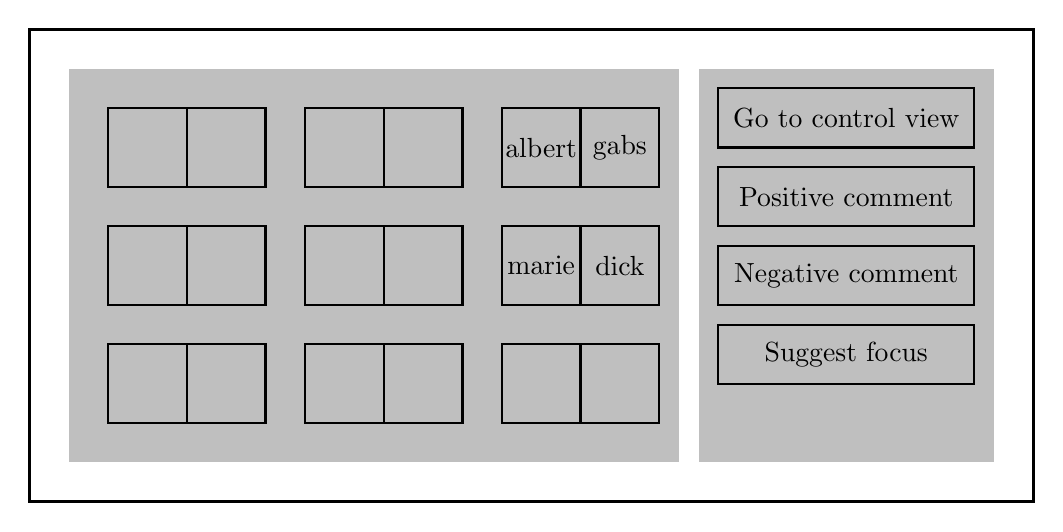
\begin{tikzpicture}

\draw[very thick] (0,0) rectangle (12.75, 6);

\fill[gray!50!white] (0.5, 0.5) rectangle (8.25, 5.5);

\foreach \x in {1, 3.5, 6} {
\foreach \y in {4, 2.5, 1} {
\draw[thick] (\x, \y) rectangle (\x+1, \y+1);
\draw[thick] (\x+1, \y) rectangle (\x+2, \y+1);
}
}

\draw[thick] (6, 4) rectangle (7, 5) node[pos=0.5] {albert};
\draw[thick] (7, 4) rectangle (8, 5) node[pos=0.5] {gabs};
\draw[thick] (6, 2.5) rectangle (7, 3.5) node[pos=0.5] {marie};
\draw[thick] (7, 2.5) rectangle (8, 3.5) node[pos=0.5] {dick};

\fill[gray!50!white] (8.5, 0.5) rectangle (12.25, 5.5);
\draw[thick] (8.75, 4.5) rectangle (12, 5.25) node[pos=0.5] {Go to control view};
\draw[thick] (8.75, 3.5) rectangle (12, 4.25) node[pos=0.5] {Positive comment};
\draw[thick] (8.75, 2.5) rectangle (12, 3.25) node[pos=0.5] {Negative comment};
\draw[thick] (8.75, 1.5) rectangle (12, 2.25) node[pos=0.5] {Suggest focus};


\end{tikzpicture}
\end{center}

Possible events: 
\begin{enumerate}
\item Pass back to the control view.
\item Change the seating plan.
\item Select/ deselect a student.
\item Record a positive comment for the selected students.
\item Record a negative comment  for the selected students.
\item Suggest students for next teacher-student focus.
\end{enumerate}

\subsection{Implementation style}
l used an object-oriented based system for the widgets that appear in the GUI, relying on inheritance and polymorphism. I quickly gave up with test-driven development, as there was too much initial investment required for this project. Indeed, as Nasser et al recently report this is a common problem when building GUIs \cite{Nass21}. The inheritance diagram of the objects used to model Buttons in the GUI is in figure \ref{inheritance_diagram_Buttons} on page \pageref{inheritance_diagram_Buttons}, and similarly a diagram for the desks is in figure \ref{inheritance_diagram_Desks} on page \pageref{inheritance_diagram_Desks}.


\begin{figure}[!hbtp] 
\begin{center}
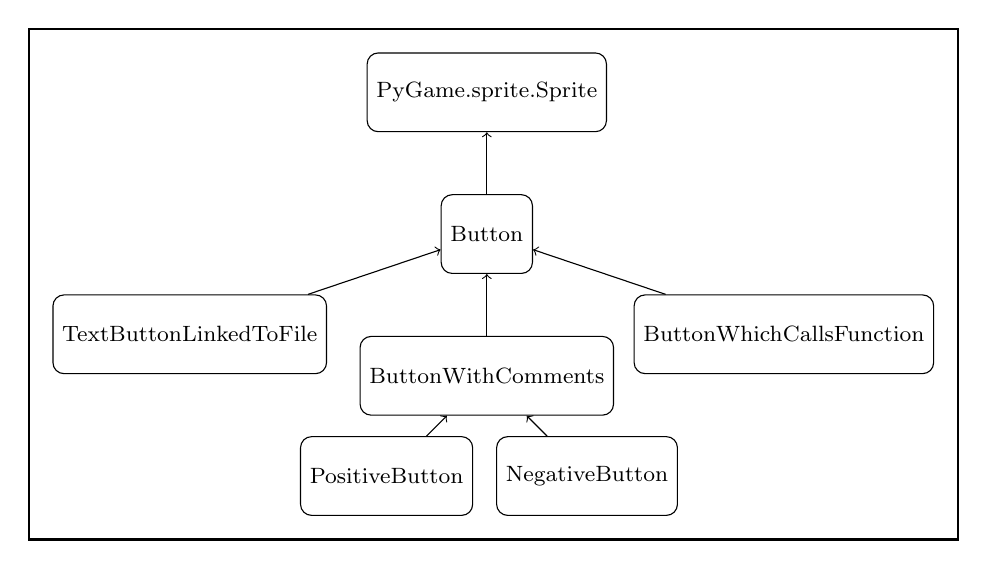
\begin{tikzpicture}[node distance=18mm, every node/.style={draw, rectangle, rounded corners, text centered, minimum height=10mm, align=center, font=\fontsize{8}{10}\selectfont}]

  % Nodes
  \node (sprite) {PyGame.sprite.Sprite};
  \node (button) [below of=sprite] {Button};
  \node (file) [below left of=button, xshift=-25mm] {TextButtonLinkedToFile};
  \node (comments) [below of=button] {ButtonWithComments};
  \node (function) [below right of=button, xshift=25mm] {ButtonWhichCallsFunction};
  \node (positive) [below left of=comments] {PositiveButton};
  \node (negative) [below right of=comments] {NegativeButton};
%  \node (shred) [below right of=comments, xshift=\datagapmm, \object] {shred comments};

  % Arrows
  \draw[->] (button) -- (sprite);
  \draw[->] (file) -- (button);
  \draw[->] (comments) -- (button);
  \draw[->] (function) -- (button);
  \draw[->] (positive) -- (comments);
  \draw[->] (negative) -- (comments);

\def\border{3mm}
\draw[thick] ([shift={(-\border,-\border)}]current bounding box.south west) rectangle ([shift={(\border,\border)}]current bounding box.north east);

\end{tikzpicture}
\end{center}
\caption{Inheritance diagram for the objects modelling the Buttons in the GUI.} \label{inheritance_diagram_Buttons}
\end{figure}


\begin{figure}[!hbtp]
\begin{center}
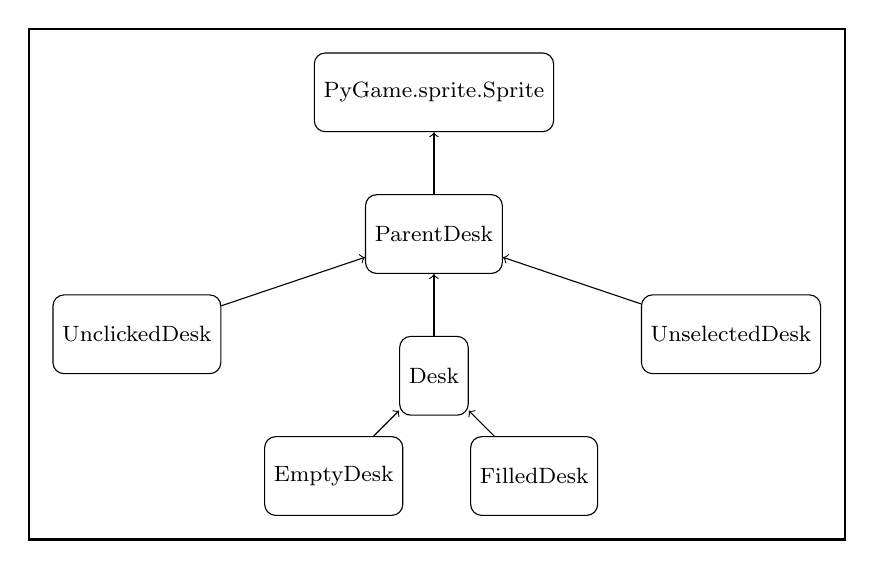
\begin{tikzpicture}[node distance=18mm, every node/.style={draw, rectangle, rounded corners, text centered, minimum height=10mm, align=center, font=\fontsize{8}{10}\selectfont}]

  % Nodes
  \node (sprite) {PyGame.sprite.Sprite};
  \node (button) [below of=sprite] {ParentDesk};
  \node (file) [below left of=button, xshift=-25mm] {UnclickedDesk};
  \node (comments) [below of=button] {Desk};
  \node (function) [below right of=button, xshift=25mm] {UnselectedDesk};
  \node (positive) [below left of=comments] {EmptyDesk};
  \node (negative) [below right of=comments] {FilledDesk};
%  \node (shred) [below right of=comments, xshift=\datagapmm, \object] {shred comments};

  % Arrows
  \draw[->] (button) -- (sprite);
  \draw[->] (file) -- (button);
  \draw[->] (comments) -- (button);
  \draw[->] (function) -- (button);
  \draw[->] (positive) -- (comments);
  \draw[->] (negative) -- (comments);

\def\border{3mm}
\draw[thick] ([shift={(-\border,-\border)}]current bounding box.south west) rectangle ([shift={(\border,\border)}]current bounding box.north east);

\end{tikzpicture}
\end{center}
\caption{Inheritance diagram for the objects modelling the Buttons in the GUI.}  \label{inheritance_diagram_Desks}
\end{figure}

\section{A single executable file} \label{executable}

Ideally, the TAT system would run from a single executable file. The user would launch the TAT application (for example, by double clicking on the icon) and then all interactions would happen through the GUI. 

I tried using two different packages: \textbf{PyInstaller}\footnote{\texttt{https://pyinstaller.org/en/stable/}} and \textbf{cx-Freeze}\footnote{\texttt{https://cx-freeze.readthedocs.io/en/latest/index.html}}. Both packages attempt to build standalone executables from Python scripts by bundling the application and dependencies into a single package. 

Importantly, both scripts are only able to build packages for the hardware and software used when building the package. This means that \textbf{I must build the executable using the school computers,} as the executable I make locally will only run on machines identical to my own. This is a clear disadvantage with the decision to use Python, a scripting language. If I had implemented the TAT system using Java, for example, then I could have assumed the school computers used a compatible virtual machine.

Unfortunately, at this time I have not managed to automate the process of creating a standalone package. PyInstaller has trouble linking to the pygame module, and cx-Freeze dislikes subfolders. Instead I manually create the executable as follows:

\begin{enumerate}
\item Create an empty folder and use this as the current directory. This can be done at the command line using

\texttt{mkdir my\_folder; cd my\_folder}

\item Copy all the TAT python scripts and the \texttt{requirements.txt} into this folder.

\vspace{1mm}

\begin{minipage}[t]{0.5\textwidth}
\begin{itemize} \scriptsize
\item TAT.py
\item control\_view.py
\item linkComments.py
\item analyseNotes.py
\item link\_gui\_backend.py
\item config.py
\item gui.py
\item students.py
\item class\_view.py
\item icons.py
\end{itemize}
\end{minipage}
\begin{minipage}[t]{0.5\textwidth}
\begin{itemize} \scriptsize
\item events.py
\item desk\_functions.py
\item constants.py
\item examNotes.py
\item shredComments.py
\item analyseComments.py
\item updateComments.py
\item scrapeClassLists.py
\item createSeatingPlan.py
\item requirements.txt
\end{itemize}
\end{minipage}

\item Create a virtual Python environment for this directory.

\texttt{python3 -m venv .}


\item Add the necessary python modules.

\texttt{pip3 install -r requirements.txt}

\item Make sure the cx-Freeze module is up to date, for example with

\texttt{ pip3 install --upgrade cx\_Freeze}

\item Again at the command line in this working directory, run cx-Freeze

\texttt{cxfreeze -c TAT.py --target-dir dist}

\item Copy the \texttt{GUI\_files} directory into the new \texttt{dist} subfolder.
\item From the \texttt{dist} subfolder, zip the following files into a single archive ready for distribution:
\begin{itemize}
\item The application file \texttt{TAT.exe}.
\item The directory of packaged files \texttt{lib}.
\item The directory of TAT options and helper files \texttt{GUI\_files}.
\end{itemize}
\item Double click on the \texttt{TAT.exe} file to launch the GUI. \\
\textbf{Warning:} the first time the application is run there is still some set up to be done, and the GUI takes a while to appear.
\end{enumerate}

\newpage
\section{Instruction booklet} \label{instructions} 

\subsection{Introducing the TAT system}
The \textbf{Teaching Assisting Tools} system, TAT, is designed to improve your teaching by automating some of the boring stuff. During class, when planning lessons, or as a reminder before meeting the parents, TAT helps manage and collate a record of your interactions with students.

\begin{center}
\begin{tcolorbox}

harry.pttr \hfill \textbf{Harry} \hfill 1ma1df01

\

\small{
01/06/2023 Harry gives conclusion of Pythag \\
01/06/2023 Harry, Ron correct calc litt \\
08/06/2023 Harry calculates hypotenuse
}

\vspace{10mm}

\begin{center}
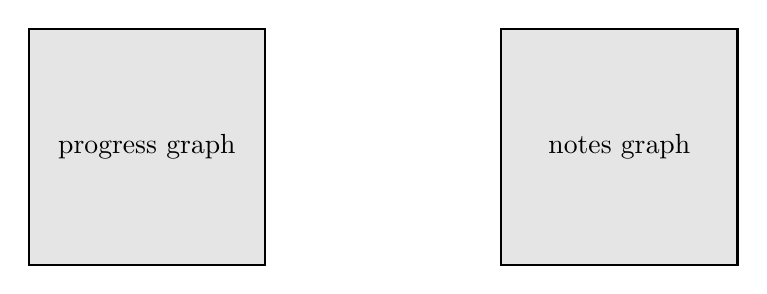
\begin{tikzpicture}

\draw[thick, fill=black!10!white] (0,0) rectangle (3,3) node[pos=0.5] {progress graph};
\draw[thick, fill=black!10!white] (6,0) rectangle (9,3) node[pos=0.5] {notes graph};

\end{tikzpicture}
\end{center}

\end{tcolorbox}
\end{center}

TAT can suggest the next students who deserve your focus during class, build individual student reports to help planning student feedback, and calculate your \emph{moyennes} over the year. In class, the tool uses a seating plan arrangement which is a very helpful reminder of names at the start of the year (and after holidays).

In the TAT folder, double-click on the icon TAT.exe to launch the program. Once TAT has started, you should see the \textbf{control view}.

\subsection{The control view}

The \textbf{control view} allows you to configure your courses and students, as well as having the system build the individual student reports and calculating all the \emph{moyennes} for you.


\begin{center}
\scriptsize
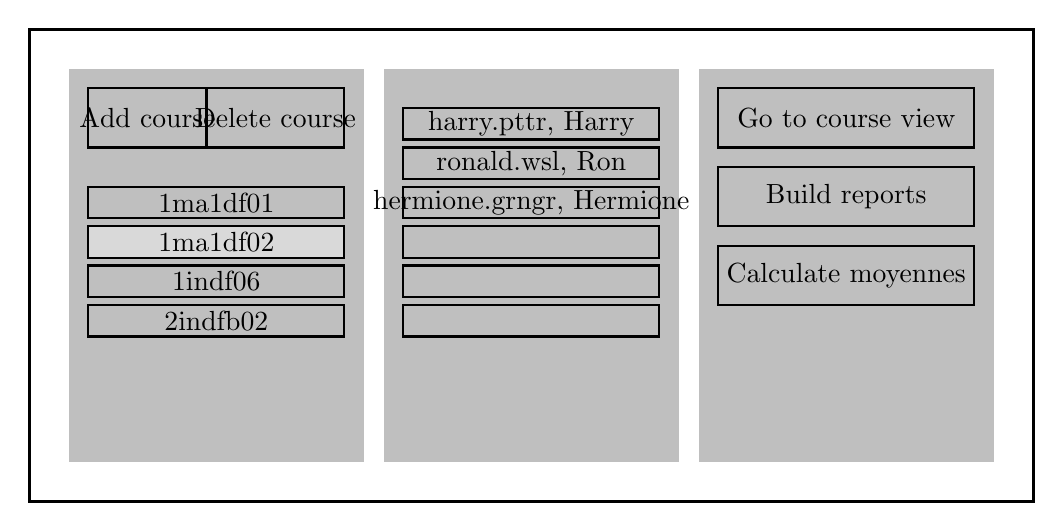
\begin{tikzpicture}

\draw[very thick] (0,0) rectangle (12.75, 6);

\fill[gray!50!white] (0.5, 0.5) rectangle (4.25, 5.5);
\draw[thick] (0.75, 4.5) rectangle (2.25, 5.25) node[pos=0.5] {Add course};
\draw[thick] (2.25, 4.5) rectangle (4, 5.25) node[pos=0.5] {Delete course};
\draw[thick] (0.75, 3.6) rectangle (4, 4) node[pos=0.5] {1ma1df01};
\draw[fill=gray!30!white, thick] (0.75, 3.1) rectangle (4, 3.5) node[pos=0.5] {1ma1df02};
\draw[thick] (0.75, 2.6) rectangle (4, 3) node[pos=0.5] {1indf06};
\draw[thick] (0.75, 2.1) rectangle (4, 2.5) node[pos=0.5] {2indfb02};

\fill[gray!50!white] (4.5, 0.5) rectangle (8.25, 5.5);
\draw[thick] (4.75, 4.6) rectangle (8, 5) node[pos=0.5] {harry.pttr, Harry};
\draw[thick] (4.75, 4.1) rectangle (8, 4.5) node[pos=0.5] {ronald.wsl, Ron};
\draw[thick] (4.75, 3.6) rectangle (8, 4) node[pos=0.5] {hermione.grngr, Hermione};
\draw[thick] (4.75, 3.1) rectangle (8, 3.5);
\draw[thick] (4.75, 2.6) rectangle (8, 3);
\draw[thick] (4.75, 2.1) rectangle (8, 2.5);

\fill[gray!50!white] (8.5, 0.5) rectangle (12.25, 5.5);
\draw[thick] (8.75, 4.5) rectangle (12, 5.25) node[pos=0.5] {Go to course view};
\draw[thick] (8.75, 3.5) rectangle (12, 4.25) node[pos=0.5] {Build reports};
\draw[thick] (8.75, 2.5) rectangle (12, 3.25) node[pos=0.5] {Calculate moyennes};


\end{tikzpicture}
\end{center}

The control view is separated into three columns : the courses you teach, the students in a selected course, and the control buttons. At the top of the first column are two buttons. The left one allows you to add a new course to the list, while the right button deletes the selected course. 

\subsubsection{Add a new course}
\textbf{Click on the "Add course" button, type the name of the course, and again click on the "Add course" button to create the course.} \\
The new course should be added as a new button in the list of courses under the "Add" and "Delete" buttons.

\subsubsection{Select a course}
\textbf{Click on the course button.} \\
The course button will turn blue, to indicate it is now the selected course. The list of students in the middle column will show the students in this course. If no students have been added yet, then the top student button helpfully reminds you that it expects \texttt{student.id, name}.

\subsubsection{Add a student to a course}
\textbf{Click on the corresponding student button, type the student.id and the name of the student (separated with a comma), and again click on the student button to save the information.} \\
Hint: the name of the student is optional. If you just enter the student.id then the TAT system will use the name in the student.id by default.

\subsubsection{Delete a course}
\textbf{First select the offending course. Now click on the "Delete course" button.} \\
This removes the course from the list of active courses. The list of students is still stored, and so you can recover a deleted course by adding it again.

\subsubsection{Build student reports}
\textbf{Click on the "Build reports" button.} \\
This will create a pdf of individual reports for each student in each class (not just the selected class). This pdf file is stored in \texttt{./latex/report.pdf} by default, and will automatically open once it has been created.

\subsubsection{Collate marks and calculate semestriel notes}
\textbf{Click on the "Calculate moyennes" button.} \\
In the spreadsheet you can adjust the weights of each exam in rows 3, 4 and 5. The rounded notes are updated automatically in the tables to the right. This xlsx file is stored in \texttt{./exams/moyennes/big\_dump.xlsx} by default, and will automatically open once it has been created.

\subsubsection{Switch to the course view}
\textbf{Select the desired course and then click on the top "Go to course" button.} \\
This will take you to the \textbf{course view}.




\subsection{The course view}

The \textbf{course view} has the seating plan on the left hand side of the view, and the control buttons on the right. The seating plan uses the ordering of the students in the course list.

\begin{center}
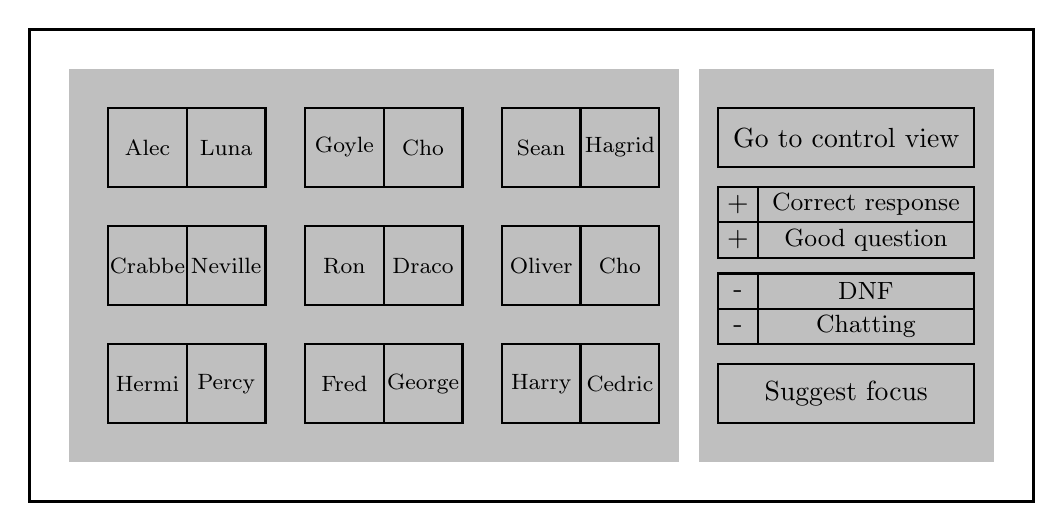
\begin{tikzpicture}

\draw[very thick] (0,0) rectangle (12.75, 6);

\fill[gray!50!white] (0.5, 0.5) rectangle (8.25, 5.5);

\def\names{{"Ginny", "Hermi", "Percy", "Crabbe", "Neville", "Alec",
  "Luna", "Fred", "George", "Ron", "Draco", "Goyle",
  "Cho", "Harry", "Cedric", "Oliver", "Cho", "Sean",
  "Hagrid", "Dumbledore", "Snape", "McGonagall", "Hedwig", "Hagrid"}}

\foreach \x in {0, 1, 2} {
\foreach \y in {0, 1, 2} {
\pgfmathtruncatemacro\index{\x*6 + \y*2 + 1}
\draw[thick] (\x*2.5+1, \y*1.5+1) rectangle (\x*2.5+2, \y*1.5+2) node[pos=0.5] {\footnotesize \pgfmathparse{\names[\index]}\pgfmathresult};
\draw[thick] (\x*2.5+2, \y*1.5+1) rectangle (\x*2.5+3, \y*1.5+2)node[pos=0.5] {\footnotesize \pgfmathparse{\names[\index+1]}\pgfmathresult};
}
}

\fill[gray!50!white] (8.5, 0.5) rectangle (12.25, 5.5);
\draw[thick] (8.75, 4.25) rectangle (12, 5) node[pos=0.5] {Go to control view};

\draw[thick] (8.75, 3.55) rectangle (9.25, 4) node[pos=0.5] {+};
\draw[thick] (8.75, 3.1) rectangle (9.25, 3.55) node[pos=0.5] {+};
\draw[thick] (9.25, 3.55) rectangle (12, 4) node[pos=0.5] {\small Correct response};
\draw[thick] (9.25, 3.1) rectangle (12, 3.55) node[pos=0.5] {\small Good question};

\draw[thick] (8.75, 2.45) rectangle (9.25, 2.9) node[pos=0.5] {-};
\draw[thick] (8.75, 2) rectangle (9.25, 2.45) node[pos=0.5] {-};
\draw[thick] (9.25, 2.45) rectangle (12, 2.9) node[pos=0.5] {\small DNF};
\draw[thick] (9.25, 2) rectangle (12, 2.45) node[pos=0.5] {\small Chatting};

\draw[thick] (8.75, 1) rectangle (12, 1.75) node[pos=0.5] {Suggest focus};

\end{tikzpicture}
\end{center}

\textbf{Note:} currently the TAT system can only handle a maximum of 24 students, sat in the standard pairs format.

\subsubsection{Modify the seating plan}
\textbf{Click and drag a student.} \\
The student will swap places with another.

\subsubsection{Select a student}
\textbf{Click on the desired student.} \\
The student will turn blue, to indicate they have been selected. Hint: you can select multiple students at once.

\subsubsection{Deselect a student}
\textbf{Click on the selected student.} \\
The student will turn yellow again. 

\subsubsection{Go back to the control view}
\textbf{Click on the "Go to control view" button at the top.} \\
This course will still be selected, so if you double click you return to the same course view.

\subsubsection{Suggest students for focus}
\textbf{Click on the "Suggest focus" button at the bottom.} \\
The TAT system will identify five students who have not received a positive comment recently and automatically select them for you (they turn blue). 

\subsubsection{Record a positive remark for students}
\textbf{Click on the corresponding "+" button.} \\
The comment next to the associated "+" button will flash red, and then all the students will be deselected. The comment has been stored, and will appear in the student reports with today's date. An example:
\begin{center}
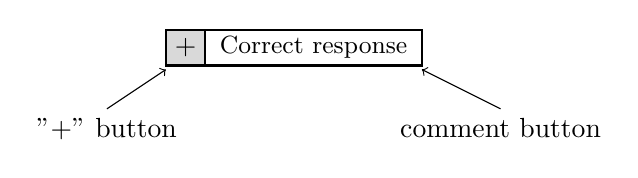
\begin{tikzpicture}

\draw[thick, fill=gray!30!white] (8.75, 3.55) rectangle (9.25, 4) node[pos=0.5] {+};
\draw[thick] (9.25, 3.55) rectangle (12, 4) node[pos=0.5] {\small Correct response};

\draw[->]  (8, 3) node[below] {"+" button} -- (8.75, 3.5);
\draw[->]  (13, 3) node[below] {comment button} -- (12, 3.5);

\end{tikzpicture}
\end{center}
These two buttons are associated. One click on the "+" button on the left will store the positive comment \texttt{"Correct response"} against all the selected students. Double-clicking on the comment button will give the same effect.

\subsubsection{Update a comment option}
\textbf{Click on the comment button, type the new comment, and click on the same comment button again.} \\
The new comment will be immediately saved for any selected students. 
Hint: the new comment is saved, and will be used next time you pass to the course view.

\subsubsection{Record a negative remark for students}
\textbf{Click on the corresponding "-" button OR double-click the comment button.} \\




\section{Missing features} \label{notdone} 

In roughly decreasing order of importance, in my opinion, here are the features I would like to see in the next implementation of the TAT system. Many of these features I had in mind as I was designing the system, but had to be descoped in this project due to time constraints.

\subsection{Handling students who leave}
In the current implementation, if a student leaves then they will soon be constantly suggested for focus. Unfortunately we cannot simply delete them from the list of students as the functions for "Shred Comments" would crash on an unknown student. This can be very annoying if, say, five students in the same class leave on an extramuros\ldots

\subsection{Button to create a blank exam file}
On the selected course, create a spreadsheet in the correct format with the student.ids already filled in. This exists in the backend but was not wired up in the GUI.

\subsection{Counting DNFs}
The backend can already count the number of \emph{devoir non fait} and return a dictionary of counts against student.ids. I did not have time to wire this into the GUI.

\subsection{Migrate to databases}
We should confirm with the PPDT\footnote{\texttt{https://www.ge.ch/organisation/protection-donnees-transparence}} what extra security would be needed, see subsection \ref{dataprivacy} on page \pageref{dataprivacy}, and migrate the system onto a database instead of flat files. This raises other needs: it would have to be easier to review and change comments on students, for example, as simply opening the \texttt{comments.txt} file would no longer be an option. Also, should we connect to the official databases for student.ids and even course lists?

\subsection{Stage the processed data}
Currently the entire raw comments file must be shredded each time the comments are used. For example, every time the system suggests students for focus it must start from the beginning even though very little (and possibly nothing) has changed since the last calculation. Intermediate steps could be saved in the database using coherent transactions which mark which data has already been preprocessed.

\subsection{Changing a name which already has comments}
Although I have yet to see this happen in reality, if a student wanted to change their given name it would cause large headaches for the current TAT system. This seems like an edge case which it should be able to handle.

\subsection{Persist seating plans}
Currently the seating plan is lost when we switch out of the class view of the GUI.

\subsection{Export seating plan to pdf}
We could plan the seating plan in advance, and then we could print it off for the students or project it on to the board.

\subsection{Suggest seating plans}
We could consider, for example, how well pairs have worked previously, or how correlated students were in exams over the different questions, or whether certain students reduce the learning around them.
\begin{center} 
\emph{``Since it has been reasonably well established that student affect toward a class is related to student learning, student attitudes toward classroom arrangements are a matter of no small concern when determining a choice of classroom arrangement.''} \cite{MM78}
\end{center}
I think a simulated annealing optimisation would work well.

\subsection{Review previous seating plans}
It would be useful to store previous seating plans.

\subsection{Configure constraints in a seating plan}
I would like to be able to take into account the needs of certain students. For example, short-sighted students often ask to sit in the front row, as do students with hearing difficulties. More rarely, students have asked to sit away from the windows because of hay-fever. These constraints could be handled by specifying particular seats as "preferable" for a given student.

Pairs of students often asked to be sat together. The decision as to whether or not these requests are accepted should rest with the teacher, but it would be a nice to have when automatically generating seating plans.

\subsection{Testing the GUI}
It is commonly accepted that it is much harder to build a testing framework for a GUI \cite{Nass21}. However, to ensure future maintainability would require either a manual Acceptance Testing process \cite[p. 53]{Amman16} or, ideally, an automated harness. The latter would require high initial investment.

\subsection{Predictions}
It would be interesting to use the data in the system to make predictions about students. For example: their behaviour in class has changed dramatically (for the better or for the worse); students who might need extra support in order to pass the year; students who should consider accelerated learning programs. There may be issues around data privacy with such an expansion though, see subsection \ref{dataprivacy}.

\subsection{Automate the process of creating a standalone package, which is currently manual}
This would be a nice to have, especially if the system was being regularly updated.




\section{Conclusion} \label{conclusion} 

The backend of the TAT system was coded using test-driven development, section \ref{tdd}, where I religiously wrote failing tests, then I wrote trivial code which passed the tests, before I finally refactored the code as much as possible. Refactoring is definitely much easier with a large suite of tests: I found I had the confidence to try much larger factorisations knowing that it was no effort to check for obvious mistakes then roll-back using version control.\footnote{I used github for this project, \url{https://github.com/danjane/GymInf}} I may be at risk of falling into a level 2 mindset of testing (testing is to show correctness), see section \ref{testing}.

However, I quickly gave up on TDD when implementing the GUI. This means that roughly half of my code was created with TDD, and half was not. I was interested to see how much better my coding would be with TDD, and so I used a Python package called \textbf{Radon} to calculate various metrics of code "goodness" \cite{Oman92}.

The Radon package analyses text-based python scripts to calculate
\begin{itemize}
\item the cyclotomic complexity of each function; roughly, the number of holes in the possible logical pathways of a function,
\item the number of lines of code, and
\item the maintainability index; a rough estimate of how easy or hard the code will be to understand, modify and maintain\cite{Oman92}. The higher the maintainability index the better, with a value in the range $[0, 100]$.
\end{itemize}
I ran the analysis on my own code base, and also calculated the average length of functions. Looking through the analysis I am not surprised to see certain functions being flagged - shredding the raw comments file was difficult to code, for example, and the PyGame loops running the GUI views involve overly long conditional chains on the events.

I was hoping to see a large difference between the code written with TDD and the rest.
\begin{center}
\begin{tabular}{|l|l|l|}
\hline
Complexities      & \textbf{Backend (TDD)} & \textbf{GUI (without)} \\ \hline
Mean            & 2.26         & 2.20             \\ \hline
Median          & 2            & 2                \\ \hline
Stdev           & 2.13         & 2.53             \\ \hline \hline
Maintainability & 49.63        & 47.53            \\ \hline
Lines of code   & 574          & 579              \\ \hline
Avg length fns     & 7.97         & 6.36             \\ \hline
\end{tabular}
\end{center}
I was surprised to see that there really is no difference as far as the metrics are concerned! Rather than being disheartened notice that the backend has a strong testing framework, making changes relatively risk free. Further, we might hope that I am becoming better at naturally refactoring as I code. 
\begin{center}
\emph{...most people who learn TDD find that \\
their programming practice changed for good.} \cite[p.xii]{Beck03}.
\end{center}
Recent research by A. Santos et al has shown that \emph{"[small projects] tend to provide less optimistic results for TDD"} and that TDD is more effective for teams.\cite{SVDU21} My aim at the start of this project was to be able to use test-driven development, not that to show that I must use TDD to write a better standard of code.

I was happy that I used Python for this project. I am also clearly more competent with PyGame, and I feel more confident replying to student questions on this package. However, I do feel that building a GUI with PyGame required a lot more work than I had expected: probably a lightweight interactive web application built with JustPy would have been more appropriate for this masters project. Another regret was that I continued to use PyCharm as my IDE: given that I was trying to improve the skills used in class, perhaps I should have used Replit or Thonny.

\

The deliverables of section \ref{deliverables} were that \emph{the TAT system will provide a basic GUI over a backend handling\ldots notes to be taken against student names and then suggest pertinent students for focus."} In this project I have managed to complete the deliverables with only a relatively small number of missing functionalities. This project has managed to "automate the boring bits", as A. Sweigart puts in \cite{Swei15}. The most recent UNESCO global education monitoring report raises the next question: what to do with all the free time I have now afforded myself?
\begin{center} 
\emph{``Technology is touted as being able to reduce the time students and teachers spend on menial tasks, time that can be used in other, educationally more meaningful activities. However, there are conflicting views on what is meaningful.''} \cite[p. 11]{Unesco23}
\end{center}

\begin{thebibliography}{Xyzz12}

\bibitem[Amman16]{Amman16} Ammann, P., \& Offutt, J. (2016). Introduction to software testing. Cambridge University Press.

\bibitem[Anaya18]{Anaya18} Anaya, M. (2018). Clean code in Python. Packt Publishing

\bibitem[Beck03]{Beck03} Beck, K. (2003). Test-driven development by example. Addison-Wesley.

\bibitem[Bloom79]{Bloom79} Bloom, B. S. (1976). Human characteristics and school learning. McGraw-Hill.

\bibitem[BCSW10]{BCSW10} Borba, P., Cavalcanti, A., Sampaio, A., \& Woodcook, J. (Eds.). (2010). Testing techniques in software engineering: Second Pernambuco Summer School on Software Engineering, PSSE 2007, Recife, Brazil, December 3-7, 2007, Revised Lectures (Vol. 6153). Springer.

\bibitem[Bryant20]{Bryant20} Bryant, J., Heitz, C., Sanghvi, S., \& Wagle, D. (2020). How artificial intelligence will impact K-12 teachers. Retrieved May, 12, 2020.

\bibitem[BS09]{BS09} Bucheton D. \& Soulé Y. (2009). Les gestes professionnels et le jeu des postures de l’enseignant dans la classe : un multi-agenda de préoccupations enchâssées.

\bibitem[Coad91]{Coad91} Coad, P., Yourdon, E., \& Coad, P. (1991). Object-oriented analysis (Vol. 2). Englewood Cliffs, NJ: Yourdon press.

\bibitem[Hat12]{Hat12} Hattie, J. (2012). Visible learning for teachers: Maximizing impact on learning. Routledge.

\bibitem[JJo20]{JJo20} Johnson, J. (2000). GUI bloopers: don'ts and do's for software developers and Web designers. Morgan Kaufmann.

\bibitem[Jorg17]{Jorg17} Jorgensen, P. C. (2017). The craft of model-based testing. CRC Press.

\bibitem[KK16]{KK16} Kelly, S., \& Kelly, S. (2016). Basic introduction to pygame. Python, PyGame and Raspberry Pi Game Development. Springer.

\bibitem[Larkin05]{Larkin05} Larkin, J. E., \& Pines, H. A. (2005). Asking Questions: Promoting student-faculty interchange in the classroom. APS Observer, 18.

\bibitem[LX10]{LX10} Lee, G., \& Xia, W. (2010). Toward agile: an integrated analysis of quantitative and qualitative field data on software development agility. MIS quarterly, 34(1), 87-114.

\bibitem[Mart08]{Mart08} Martin, R. (2008). Clean Code. Pearson.

\bibitem[Mart17]{Mart17} Martin, R. (2017). Clean Architecture: A Craftsman’s Guide to Software Structure and Design. Pearson

\bibitem[Mart11]{Mart11} Martinez, W. L. (2011). Graphical user interfaces. Wiley Interdisciplinary Reviews: Computational Statistics, 3(2), 119-133.

\bibitem[MM78]{MM78} McCorskey, J. C., \& McVetta, R. W. (1978). Classroom seating arrangements: Instructional communication theory versus student preferences. Communication education, 27(2), 99-111.

\bibitem[MSB11]{MSB11} Myers, G. J., Sandler, C., \& Badgett, T. (2011). The art of software testing. John Wiley \& Sons.

\bibitem[Nass21]{Nass21} Nass, M., Alégroth, E., \& Feldt, R. (2021). Why many challenges with GUI test automation (will) remain. Information and Software Technology, 138, 106625.

\bibitem[Norm13]{Norm13} Norman, D. (2013). The design of everyday things: Revised and expanded edition. Basic books.

\bibitem[Norr98]{Norr98} Norris, J. R. (1998). Markov chains (No. 2). Cambridge university press.

\bibitem[Oman92]{Oman92} Oman, P., \& Hagemeister, J. (1992, January). Metrics for assessing a software system's maintainability. In Proceedings Conference on Software Maintenance 1992 (pp. 337-338). IEEE Computer Society.


\bibitem[PPDT18]{PPDT18} Le PPDT - Guide pratique RGPD à l'attention des institutions publiques genevoises (2018).

\bibitem[Raj2018]{Raj2018} Raj, A. G. S., Patel, J. M., Halverson, R., \& Halverson, E. R. (2018, November). Role of live-coding in learning introductory programming. In Proceedings of the 18th koli calling international conference on computing education research (pp. 1-8).

\bibitem[Rob19]{Rob19} Robinson, M. (2019). BOSCARD: A Scoping Tool for Lean Continuous Improvement Projects. In Global Lean for Higher Education (pp. 181-195). Productivity Press.

\bibitem[Rowe74]{Rowe72} Rowe, M. B. (1974). Wait-Time and Rewards as Instructional Variables: Their Influence on Language, Logic, and Fate Control. Journal of research in science teaching, 11(2), pp. 81-94.

\bibitem[SVDU21]{SVDU21}Santos, A., Vegas, S., Dieste, O., Uyaguari, F., et al (2021). A family of experiments on test-driven development. Empirical Software Engineering, 26, 1-53.

\bibitem[Swei15]{Swei15} Sweigart, A. (2015). Automate the Boring Stuff with Python.

\bibitem[Tidw10]{Tidw10}Tidwell, J. (2010). Designing interfaces: Patterns for effective interaction design. O'Reilly Media, Inc.

\bibitem[Unesco23]{Unesco23} UNESCO (2023). Global Education Monitoring Report: Technology in education: a tool on whose terms? Paris: UNESCO.

\bibitem[Viau94]{Viau94} Viau, R. (1994). La motivation en contexte scolaire. Éditions du Renouveau pédagogique.

\end{thebibliography}

\appendix

\section{Original project proposal}

Bucheton and Soulé have described the act of teaching as a multi-agenda game of postures requiring good preparation and excellent micro-decisions \cite{BS09}. In their model, they identify the crucial roles of the teacher in controlling the cadence, the atmosphere, the scaffolding and the relationships during the class, and how each supports the learning objective. And yet many of the teacher's most time-consuming tasks do not take place in the classroom \cite{Bryant20}: good preparation and strong follow-ups (for example auto-reflection, marking and parent-teacher interactions) work to support and complement the pillars identified in the student learning process.

Many of these tasks are ripe for automation. As Sweigart writes, ``many people spend hours clicking and typing to perform repetitive tasks, unaware that the machine they’re using could do their job in seconds if they gave it the right instructions'' \cite{Swei15}.  For my thesis project of the GymInf formation, I intend to build a suite of tools to support a range of teacher tasks including 
\begin{itemize} 
\item organizing seating plans \\
\emph{to aid the atmosphere and relationships} 
\item suggesting teacher-student interactions for upcoming classes \\
\emph{to foster relationships}
\item building individual student reports \\
\emph{to regulate cadence and scaffolding, as well as for follow-ups}
\item creating spreadsheets of marks \\
\emph{for follow-ups}
\end{itemize}
Teachers will interact with the tool using a GUI: it should be easy to use for all teachers, not just those teachers who are computer literate.


I will implement this project using \emph{Test-Driven Development.} This is a style of software development that grew out of the `Extreme Programming' philosophy of the 1990s, encouraging quick development cycles and active feedback from clients. The first book written on the subject, \emph{TTD by Example}, by Kent Beck, is still the main resource \cite{Beck03}. Kent emphasises the need to thoroughly test the requirements in order to have confidence when refactoring or making changes, as well as the need to make incremental changes (both for confidence and for time to market). TTD programming follows the following cycle: \\
\indent \textbf{Red.} Write a failing test for a requirement. \\
\indent \textbf{Green.} As quickly as possible, write code to pass the test. \\
\indent \textbf{Refactor.} Clean the code, removing duplication and renaming functions. \\
Coding is driven by testing. In the thesis I will explore testing in more detail.



\end{document}